\documentclass[a4paper, % papirstørrelse, skal altid med
final,% Når man skal skifte kompileringsmetode mellem draft og final skal man 
      %flytte kommenteringen %  i Draft kommanoerne, nedenfor.
11pt, % standardstørrelse på fonten
openany%, % anvnedes hvis kapitler bare skal starte på den næste side
%oneside,
%article
]{memoir}%
% marginer, memoir to to metoder
% den traditionelle, se memoir manualen
% venstre: 2.5cm, højre: 3.5cm, top: 3cm, bund: 4cm
%her kan margenen sættes manuelt, hvis man har lyst
%\setlrmarginsandblock{3.5cm}{3.5cm}{*}
%\setlrmarginsandblock{1.5cm}{6.5cm}{*}
%her kan margenen sættes manuelt, hvis man har lyst
%\setulmarginsandblock{3cm}{4cm}{*}
% % mere utraditionelt, men hurtigt smartere
% % vi sætter tekstblokken og placerer den
% % værdierne som er angivet svarer ca. til dem anvende i LaTeXbogen
% % 400pt bred og en højde svarende til at forholdet er det gyldne snit
%\settypeblocksize{*}{300pt}{1.618}
% % placer tekstblokken på papriet, kun en værdi skal angives, her sider
% % vi bare hvad forholder mellem marginerne skal være
% \setlrmargins{*}{*}{1.6}
% \setulmargins{*}{*}{1.3}
\checkandfixthelayout % laver forskellige beregninger og sætter de
% almindelige længder op
\usepackage[utf8]{inputenc} % eller utf8 eller ansinew eller ...
\usepackage[danish]{babel} %direktiv til at bruge det danske sprog

\usepackage[draft]{fixme} % til at skrive \fixme kommentarer til sig

%\newenvironment{Draft}{\fixme{HUSK at ændre kommenteringen i preamble når man skifter mellem draft og final} }{  }
\let\Draft=\comment \let\endDraft=\endcomment


%har vi ord der bliver delt forkert kan de indsættes i hyphernation med bindestreg alle steder hvor ordet kan deles
\hyphenation{tit-len mo-del-len pro-du-ce-rer an-svars-hav-ende om-for-deles for-bind-elses-mulig-heder ska-ber æn-dring-er net-værks-en-hed-er peer backup backup-system fast-track backup-systemer nabo-peers frame-work efter-som Grund-lag-et plads-effek-tivi-teten audits}


\usepackage{nameref}
\usepackage[danish]{varioref} % smarte krydsreferencer via \vref
\usepackage[colorlinks, linkcolor=blue, citecolor=blue, urlcolor=blue, 
final=true]{hyperref}

%giver mulighed for at hoppe i pdf'filen via referencerne.
%hyperref er ustabil med varieof,
%og skal udkommenteres hvis der opstår problemer.
%specielt skal udkommenteres når man kompilere i final til print

\renewcommand\danishhyphenmins{22} % bedre orddeling
\addto\captionsdanish{%brug bedrer danske ord for de faste tekster
\renewcommand\contentsname{Indholdsfortegnelse}
\renewcommand\appendixname{Appendiks}
}

\usepackage{csquotes}
\usepackage[style=numeric-comp,sorting=nyt]{biblatex}
\DefineBibliographyStrings{danish}{%
references      = {Litteraturliste},
bibliography    = {Litteraturliste},
urlseen         = {Lokaliseret d\adddot},
andothers 		= {m\adddot fl\adddot},
typeeditor      = {{udgiver}{udg\adddot}},
typeeditors 	= {{udgivere}{udg\adddot}},
}

\usepackage[T1]{fontenc} % bedre orddeling og ofte påkrævet at
% forskellige fonte
%\usepackage{fourier} % eller mathpazo eller lignende, eller fjern den
% for at få standard fonten
% sætter nogle default værdier vedr. floats

\let\newfloat\relax % memoir har allerede defineret denne men det gør
% float pakken også
\usepackage{float}
\restylefloat{table}
\floatevery{table}{\centering\small} % alle tabel floats centreres og
% skrives i \small
\restylefloat{figure}
\floatevery{figure}{\centering} % automatisk centrering af alle
% figurer
% float environments får ’htbp’ som standard placerings værdier når
% man ikke har angivet noget

\makeatletter
\renewcommand\fps@figure{htbp}
\renewcommand\fps@table{htbp}
\makeatother
\usepackage{amsmath,amssymb} % bedre matematik og ekstra fonte
\usepackage{textcomp} % adgagn til tekstsymboler
\usepackage[notcite,notref]{showkeys} % viser labels i margin,
% udkommenteres for at fjerne, eller
% anvend option final


\setsecnumdepth{subsubsection} % eller hvor dybt man nu ønsker at har
% overskrifterne nummereret
\maxsecnumdepth{subsubsection}
\settocdepth{subsubsection} % hvor dybt ned vi ønsker ting med i

% OPSÆTNING AF SÆTNINGER etc.
\usepackage[amsmath,thmmarks]{ntheorem} % bedre fleksimibitet
\usepackage[final]{graphicx} % pakke til inklusion af grafik
\usepackage{epsfig}

\makeindex % hvis man ønsker at lave et index
%\usepackage{pstricks}
\usepackage{tikz}


%Linjeafstand: (1,5 = siderne bliver ca. til ns)
\linespread{1,5}
\selectfont

\newcommand{\des}[0]{Discrete event simulation}

% OPSÆTNING TIL INKLUDERING AF SOURCE CODE
\usepackage[final]{listings}
\usepackage{courier}
 \lstset{
         basicstyle=\footnotesize\ttfamily, % Standardschrift
         %numbers=left,               % Ort der Zeilennummern
         numberstyle=\tiny,          % Stil der Zeilennummern
         %stepnumber=2,               % Abstand zwischen den Zeilennummern
         numbersep=5pt,              % Abstand der Nummern zum Text
         tabsize=2,                  % Groesse von Tabs
         extendedchars=true,         %
         breaklines=true,            % Zeilen werden Umgebrochen
         keywordstyle=\color{red},
                frame=b,         
 %        keywordstyle=[1]\textbf,    % Stil der Keywords
 %        keywordstyle=[2]\textbf,    %
 %        keywordstyle=[3]\textbf,    %
 %        keywordstyle=[4]\textbf,   \sqrt{\sqrt{}} %
         stringstyle=\color{white}\ttfamily, % Farbe der String
         showspaces=false,           % Leerzeichen anzeigen ?
         showtabs=false,             % Tabs anzeigen ?
         xleftmargin=17pt,
         framexleftmargin=17pt,
         framexrightmargin=5pt,
         framexbottommargin=4pt,
         %backgroundcolor=\color{lightgray},
         showstringspaces=false      % Leerzeichen in Strings anzeigen ?        
 }
 \lstloadlanguages{% Check Dokumentation for further languages ...
         %[Visual]Basic
         %Pascal
         %C
         %C++
         %XML
         %HTML
         PYTHON
 }
    %\DeclareCaptionFont{blue}{\color{blue}} 

  %\captionsetup[lstlisting]{singlelinecheck=false, labelfont={blue}, textfont={blue}}
  \usepackage{caption}
\DeclareCaptionFont{white}{\color{white}}
\DeclareCaptionFormat{listing}{\colorbox[cmyk]{0.43, 0.35, 0.35,0.01}{\parbox{\textwidth}{\hspace{15pt}#1#2#3}}}
\captionsetup[lstlisting]{format=listing,labelfont=white,textfont=white, singlelinecheck=false, margin=0pt, font={bf,footnotesize}}




\usepackage{pdfpages}

%\includeonly{../litteratur}





\bibliography{bibliography} %indsaet en reference til bib filen

%\includeonly{interactive/interactive}
\begin{document}
\pagenumbering{Roman} 
\begin{titlingpage}
\newcommand{\HRule}{\rule{\linewidth}{1mm}}
\vspace*{\stretch{1}}
\noindent\HRule
\begin{flushright}
                \large 
                Rasmus Sørensen\\
                Simon Bognolo
                \\[5mm]
            \huge \Title
\end{flushright}                
\HRule
\vspace*{\stretch{2}}
\begin{center}
\large\textsc{maj 2010}\\
\large\textsc{Datalogisk Institut, Københavns Universitet}
\end{center}
\end{titlingpage}

\frontmatter
\begin{otherlanguage}{english}
\thispagestyle{empty}
  \begin{abstract}

Over the last years, multi-core cpu's have become increasingly more common, which has lead to a demand for easy representation of concurrency in application development. This has increased the popularity of CSP, leading to implementations in several common programming languages. 

Most practical representations of time in CSP currently breaks with the CSP paradigm, so in this thesis we will explore the possibilities of including a representation of time directly in an implementation of CSP. The goal is to make one or several representations of time that gives a developer the tools needed to handle problems within a timecentric domain. We limit ourselves to uses of time within discrete event simulation, real time planning and interactive planning. For each use we approach the problem using applicable examples to identify key issues and requirements. 

We have found that representations of time in applications are not bound to their problem domain, but rather the time model they apply. As such we have developed two representations of time, one using discrete time, the other using real time. 

%Our representation of discrete time meets all identified demands for application in discrete event simulations. We provide an intuitive and flexible solution, that ... 

%Realtime planning and interactive planning have been joined in one representation as they share time model. The model uses the Earliest Deadline First (EDF) algorithm to prioritize events, with added priority inheritance to handle priority inversion. 

Our solution provides developers with intuitive and flexible representations of time, allowing them to focus more on the actual problem, and less on representation and management of time.\\
\\
The implementation can be found at the address given below. The code specific for this thesis is located in \href{http://code.google.com/p/pycsp/source/browse/\#svn/branches/TimedPyCSP/pycsp/simulation}{\texttt{/pycsp/simulation}} and \href{http://code.google.com/p/pycsp/source/browse/\#svn/branches/TimedPyCSP}{\texttt{/pycsp/deadline}}. \\
\url{http://code.google.com/p/pycsp/source/browse/\#svn/branches/TimedPyCSP}\\
\\
The examples used in the thesis are located at the address given below, and can also be found in the appendix.\\
\url{http://github.com/shamran/TimedPyCSP/tree/master/projects}
\end{abstract}
\end{otherlanguage}
%\begin{abstract}
%  bla bla (på dansk)
%\end{abstract}


\tableofcontents
\newpage

\listoffixmes
\newpage
\lstlistoflistings   
\newpage

%\savepagenumber

%\chapter{Tidsplan}
Når et kapitel er færdig skal det læses igennem af os begge og gennemdiskuteres.
\begin{list}{}{}
\tightlist 
\item [8/2] \des færdig.
\item [20/2-28/2] Vinterferie.
\item [29/2] \ds færdig.
\item [3/5] \is færdig.
\item [10/5] Første fulde gennemlæsning færdig, med fokus på sammenhæng af kapitlerne
\item [14 dage buffer.]
\item[25/5] Undersøg med informationen om de har åbent d. 31/5.
\item [25/5-27/5] Sidste gennemlæsning færdig med fokus på små rettelser.
\item [27/5 -30/5] sidste opsætning, printning, og indbinding.
\item [31/5] Aflevering. 
\end{list}\
\begin{tabular}{m{0.5cm}m{4cm}}
\hline  
\multicolumn{2}{m{4.5cm}}{\textbf{Status på \des:}} \\
\hline
100\% & Kode.  \\ 
70\% & Eksempler.\\
0\% & Beskrivelse og Teori.\\
0\% & Design og  implementering. \\
0\% & Evaluering. \\
0\% & Fremtidigt arbejde. \\
0\% & Opsummering. \\ 
\hline
\end{tabular}
\quad
\begin{tabular}{m{0.5cm}m{4cm}}
\hline  
\multicolumn{2}{m{4.5cm}}{\textbf{Status på Deadline scheduling:}} \\
\hline
0\% & Kode.  \\ 
0\% & Eksempler.\\
0\% & Beskrivelse og Teori.\\
0\% & Design og  implementering. \\
0\% & Evaluering. \\
0\% & Fremtidigt arbejde. \\
0\% & Opsummering. \\ 
\hline
\end{tabular}\\
\begin{tabular}{m{0.5cm}m{4cm}}
\hline  
\multicolumn{2}{m{4.5cm}}{\textbf{Status på interaktive scheduling:}} \\
\hline
0\% & Kode.  \\ 
0\% & Eksempler.\\
0\% & Beskrivelse og Teori.\\
0\% & Design og  implementering. \\
0\% & Evaluering. \\
0\% & Fremtidigt arbejde. \\
0\% & Opsummering. \\ 
\hline
\end{tabular}
\subsection*{Ugentlige deadline}
\textbf{Deadline d. 18. jan.}
\begin{itemize}{}{}\tightlist
\item Skrevet barrierer afsnit færdigt, så det er generisk og kan bruges af begge eksempler.
\item Wator overordnet og Wator uden tid skal være færdig.
\item Bank overordnet og uden tid skal være færdigt.
\item Simon skal have begyndt på design og implementering.
\end{itemize}
\mainmatter
%\SingleSpacing
\DoubleSpacing
%\OnehalfSpacing
\selectfont 
%%%%%%%%%%%%%%%%%%%%%%%%%%%%%%%%%%%%%%%%%%%%%%%%%%%%%%%%%%%%%%%%%%%%%%
\chapter{Introduktion}
  \section{Problem}	 
  \section{Kontekst - Baggrund og motivation}
Over de siste par år er multi-kerne cpu'er blevet hyldevarer, og er at finde i 
stort set alle computere det sælges nu om dage. For at udnytte den ekstra 
ydelse der er til rådighed med flere kerner, er softwareudviklere nødt til at 
ændre på tankegangen og metoderne der hidtil har været brugt til at udvikle 
programmer. Hvor man tidligere har kunne udvikle programmer ud fra en meget 
sekventiel tankegang, er man nu nødt til at muliggøre samtidig afvikling af 
opgaver, således de kan udnytte flere kerner samtidigt. Dette stiller både krav 
til udviklerne og de værktøjer og sprog de benytter til udvikling.  En metode 
til at repræsentere den krævede samtidighed på, er ved hjælp af 
CSP\cite{hoare-csp}.  I CPS opdeles et program i selvstændige processer, der 
kan afvikles samtidigt på hver sin kerne. Der bør som udgangspunkt ike være 
delt data mellem processer, og al kommunikation mellem processer sker eksplicit 
via kanaler. Dette gør det let at overskue og meget egnet til multi-kerne 
arkitekturer. Ydermere lægger det op til at komplekse systemer opbygges af 
mindre individuelle enheder, og kobles sammen med kanaler for så til sammen at 
udgøre systemet som helhed.
Opdelingen af et program i processer skaber nye problemstillinger, som ikke er 
til stede i sekventielle programmer. Specifikt introduceres der et behov for 
synkronisering af processerne idet de ofte vil have en indbyrdes afhængighed af 
større eller mindre grad. Denne synkronisering kan ske implicit eller eksplicit 
i programmet, afhængig af strukturen i det givne program. Ved eksplicit 
synkronisering forstås at der er i programmet findes elementer hvis primære 
formål er at håndtere synkronisering. Ved implicit synkronisering sker 
synkroniseringen ud fra programmets normale kommunikation mellem processerne, 
og ingen ekstra elementer til håndtering af synkronisering er nødvendige.  

\subsection{usammenhængende råtekst}
Der er, så vidt vi ved, ikke nogen tilgængelige implementationer af CSP der 
tager... 

CSP er tilgængeligt som en udviddelse til en række sprog, heriblandt Java, C++ 
og Python. I Python hedder udviddelsen PyCSP, og er udviklet i et samarbejde 
mellem mellem Tromsø og Københavns Universitet, med henblik på at skabe et 
sprog som er let forståeligt men samtidigt giver den påkrævede mulighed for 
repræsentation af samtidighed.  


Af de implementationer af CSP der findes på nuværende tidspunkt, er der, så 
vidt vi ved, ingen der har en reel repræsentation af tid indbygget. Det gør at 
tidsspecifikke programmer, som f.eks. realtids-simuleringer, kræver brug af 
andre konstruktioner i sproget.
Vi ønsker at undersøge muligheden for at introducere tid som en indbygget del 
af PyCSP for derved at kunne lette implementationen af programmer der i større 
eller mindre grad er bundet op omkring et tidselement. k


I sin nuværende form kræver styring af tid i PyCSP brug af 
barrierer\inline{generelt term eller henvisning til MPI?}. Dette skaber et 
behov for flere kanaler mellem de enkelte processer og de fornødne barrierer, 
samt kald til en barriere når en proces skal vente på at fortsætte.  Dette 
resulterer som helhed i mindre overskuelig kode, hvilket vi mener kan gøres 
mere elegant med indbygget funktionalitet til håndtering af tid. Målet er at 
give mulighed for at integrere relationen til tid direkte i det udviklede 
program, i stedet for at benytte 


  \section{Fremgangsmåde}
  \section{``Summary of contributions''}
  \section{Termer}

\begin{list}{}{}

\item Scheduler findes ikke som et dansk ord, som kan  dække helt det samme. Vi har valgt at bruge ordet skemaplanlægger.
\item I \des beskriver det enkelte \code{event} en begivenhed, og vi vil i dette speciale bruge ordet begivenhed for en event i \des. 
\item realtid: tid mål i sekunder, minutter osv.
\item event: begivenhed
\item Vi har fra koden der vises fjernet kode der ikke er relevant for sammenhængen, som f.eks kald til logging. Linje nr. vil derfor ikke altid passe, men det første linje nr i kodestumpen vil svare til linjenr i source koden.
\end{list}



nu med test teswt

nu med mere tes


meret

\chapter{Simulering i diskret tid}
\inline{sammenligning af simulation vs. modellering.\\
  simulering er en implementation af modellen.\\
  styrke er samspillet mellem flere elementer/modeller.\\
  simulering - dynamisk - tid (time/space).} 
\pdfcomment{Hvad skal der foregå i dette kapitel? Hvorfor? og evt. hvordan?}
Vi vil i dette kapitel gennemgå hvad computersimuleringer kan bruges til, med fokus på discrete event simulation (\des). Indenfor \des vil vi redegøre for hvilke problemstillinger vi skal tage højde for, for at kunne implementere en \des tidsmodel i \pycsp. 

Simuleringer har længe været et værdifuldt værktøj til at klarlægge hvordan et system fungerer og er specielt brugbart til at repræsentere systemer hvis 
tilstand ændres over tid, eller såfremt der er interaktion mellem flere systemer. Tabel \ref{tab:simulation_examples} viser domæner hvor simulering ofte bruges som løsningsmodel. 

DES bruges meget i forbindelse med BI hvor erhvervsfolk f.eks ønsker at få klarlagt hvordan produktionen ser ud på en fabrik. Det kan også bruges i forskningsverdenen til komplekse repræsentationer af kemiske eller fysiske processer der ændrer sig over tid. 
Generelt bruges simuleringer til at forudse hvor hvordan en eventuel ændring af systemet vil påvirke systemet som helhed. Dette vil typisk også kunne opnås med en matematisk model over systemet, men denne vil være væsentlig mere kompleks og sværere at overskue. 

find reference der snakker om matematisk model vs simulering. 


\begin{table}[ht]
	\begin{tabularx}{\textwidth}{|p{15pt}Xp{15pt}|p{15pt}Xp{15pt}|}
  \hline  
  &&&&&\\
  \multicolumn{3}{|c|}{\textbf{General Situation}}&\multicolumn{3}{c|}{\textbf{Examples}} \\
  &&&&&\\  
  \hline
  & \vspace{5pt}Real system does not yet exist and building a prototype is cost prohibitive, time-consuming or hazardous. \vspace{5pt}& & & \vspace{5pt}Aircraft, Production System, Nuclear Reactor \vspace{5pt}& \\
  \hline  
  & \vspace{5pt}System is impossible to build.\vspace{5pt} & & & \vspace{3pt}National Economy, Biological System\vspace{5pt} &\\
  \hline
  & \vspace{5pt}Real system exists but experimentation is too expensive, hazardous or disruptive to conduct.\vspace{5pt} & & & \vspace{5pt}Proposed Changes to a Materials Handling System, Military Unit, Transportation System, Airport Baggage Handling System\vspace{5pt} & \\
  \hline
  & \vspace{5pt}Forecasting is required to analyze long time periods in a compressed format.\vspace{5pt} & & & \vspace{5pt}Population Growth, Forest Fire Spread, Urbanization Studies, Pandemic Flu Spread \vspace{5pt}&\\
  \hline
  & \vspace{5pt}Mathematical modeling has no practical analytical or numeric solution.\vspace{5pt} & & & \vspace{5pt}Stochastic Problems, Nonlinear Differential Equations\vspace{5pt} & \\
  \hline	
  \end{tabularx}
	\caption{Anvendelsesområder for simuleringer. Tabellen er kopieret fra \cite[10]{Mchaney2009}}
	\label{tab:simulation_examples}
\end{table}



\section{Beskrivelse/teori} \label{sec:des-teori}
\inline{Beskrivelse af tidsmodellen, teorien omkring den og hvor/hvad den 
    benyttes til. Teori: henvisning til litteratur, bl.a.  matematik/beviser 
    for modellen}
\inline{Skal vi skrive noget om at introduktionen af tid er det samme som at introducere prioritet}

\begin{shaded}
\fxnote{Gennemlæses og højst sandlysningt omskrives med henblik på sammenhæng og mangler.}
Indenfor simulering er \des en meget brugt metode til at modellere systemer. I 
\des anskues tid som diskrete tidsskridt som er uden kobling til realtid. I 
disse tidsskridt udføres en eller flere begivenheder, som hver især ændrer på systemets tilstand. Når alle begivenheder for et tidsskridt er udført kan tiden tælles op og begivenheder for det nye tidsskridt kan udføres. Der kan være være planlagt et vilkårligt antal beginvenheder til et tidsskridt og hver begivenhed kan variere vilkårligt med henlik på hvor langt tid den tager at udføre i realtid. Det er disse betingelser der forårsager at der ikke er nogen kobling mellem den diskrete tid og realtid, og et diskret tidsskridt kan derved variere arbitrært i realtid. Begivenhederne der skal udføres af systemet kan enten være givet på forhånd, eller blive skemaplanlagt dynamisk under afviklingen af andre begivenheder. 
Afhængig af hvad der simuleres, kan man udtrække relevant information om systemet, f.eks. gennemsnitlig behandlingstid for elementer, længden af køer i systemet, og den samlede aktivitetstid for hvert delelement i systemet.


For at kunne konstruere en \des skal vi have følgende til rådighed; En repræsentation af tid til at styre hvornår vi skifter tidsskridt, en liste over begivenheder der skal udføres i hvert tidsskridt, samt mulighed for at opsamle statistisk data fra simulationen. 

    
I \csp har vi garanti for at de eneste afhængigheder mellem processer vil være kommunikation. I \des har vi ud over kommunikation også en afhængighed af at synkronisere tiden mellem processerne.En simulering løber begivenhederne kronologisk igennem til der enten ikke er flere begivenheder eller som det oftere er tilfældet til simuleringen når et forud defineret tidspunkt.

\fxnote*[inline,nomargin]{Brian: ok brug af parallelitet}{Alternativet til  \des  er \pdes hvor tiden i processerne kan løbe uafhængigt af hinanden. Dette introducerer muligheden for større parallitet, men samtidigt risikerer processerne ved kommunikation at modtage beskeder fra fortiden, som der skal tages hånd om, f.eks. ved at rulle tiden tilbage. \pdes har ikke vundet stort indpas i den videnskabelig verden som man kan se af \cref{tab:des}, en grund til dette er at når tiden kan køre parallelt vil de deraf følgende omkostningerne resultere i lavere hastighed end ved at holde tiden synkront på tværs af processerne.}
\end{shaded}
\begin{table}[ht]
	\centering
	\begin{tabular}{lrr}
	\toprule
	\mc{Periode} & \mc{DES} & \mc{PDES}\\
	\midrule
1970 til 1980 &   296 &2\\
1980 til 1990 & 1.460 &95\\
1990 til 2000 & 6.190 &1.260\\
2000 til 2010 &13.100 &1.210\\
\bottomrule
	\end{tabular}
	\caption{Publisering af artikler if. google scholar ved søgning på hhv. ''\des'' og ''parallel \des''}
	\label{tab:des}
\end{table}
\subsection*{Noter til afsnittet}
\begin{itemize}
\tightlist
	\item stokastisk varians i relation til M/M/1
	\item Hvad bruges DES til? styrker/svagheder?
	\item Henvis til DE-simulation.ps
\end{itemize}


\subsection{Barrierer} \label{sec:barrierer}
%\inline{Hele afsnittet skal skrives om for at få det generelle samlet i starten, og vores specifikke efterfølgende. Evt. have mindre om vores implementation}

I \des findes der  en global tid og alle processerne skal derfor have en fælles tid der tæller op 
samtidigt.  En global viden som tid kræver synkronisering af alle 
processerne, og til denne koordinering og synkronisering af flere 
processer er  den mest brugte metode at introducere en barriere. Barrierer blev først introduceret i MPI \cite{mpi-barrier}, hvor den bruges til at 
sikre at alle tråde venter i barrieren før de kan fortsætte. 

I \csp kan man lave sin egen barrierer ved at udnytte at begge 
kanalender skal være klar, før der der kan kommunikeres og at en proces der er 
indgår i en kommunikation vil vente indtil den anden ende er klar før den 
fortsætter.  Ved hjælp af kanaler kan man derfor lave en simpel barriere 
trivielt ved brug af kommunikation over kanaler.  En implementering af en 
barriere som en selvstændig proces kan ses i 
\cref{barrier-imp}.

\begin{lstlisting}[float, label=barrier-imp,caption=En barriere i \pycsp]
@proces
def Barrier(nprocesses, signalIN, signalOUT):
	while True:
		for i in range (nprocesses):
			signalIN()
		for i in range (nprocesses):
			signalOUT(0)
\end{lstlisting}
%
%Denne implementering af en barriere kræver, i modsætning til de fleste andre 
%implementeringer af barrierer\cites{mpi-barrier, crew}, to kald. Det første 
%sender en variabel til barriereprocessen, mens,
%det andet kald modtager en dummyværdi fra barriereprocessen. Det kræver derved 
%to kanaler at implementere barrieren. På den ene kanal er barrieren den eneste 
%der læser værdierne; en besked sendt på denne kanal vil derfor altid modtages 
%af barrieren. På den anden kanal er barrieren den eneste der skriver, og en 
%modtaget besked må derfor komme fra barrieren.
%
%Vi kan overbevise os om korrektheden af barrieren, da alle processerne først 
%går ind i barrieren ved at sende en værdi til barrieren. Hvis barrieren ikke er 
%klar, sikrer \csp at processerne venter indtil barrieren er klar til at modtage 
%værdierne. Først når barrieren har modtaget en værdi fra alle processerne, 
%begynder barrieren at sende sin værdi, og det er først når en proces modtager 
%denne værdi fra barrieren at den må fortsætte. Når en proces modtager værdien 
%fra barrieren fortsætter den og man kan risikere at den ønsker at gå ind i 
%barrieren inden denne har sendt sin værdi til alle processer for at frigive dem.
%Processer der ønsker adgang til barrieren vil da gå i stå, idet de prøver at 
%sende til barrieren før den er klar til at modtage. Først 
%når barrieren har signaleret til alle processer at de må fortsætte, læser den 
%på kanalen for at accepterer processer der ønsker at tilgå barrieren. Det er 
%denne egenskab fra \csp der giver os garanti for at en proces der netop er 
%frigivet fra barrieren ikke går ind i den igen og derved risikerer at komme 
%foran. 
%
%En ulempe ved denne simple barriere er at antallet af processer skal være 
%konstant gennem hele kørslen.
%Vi vil senere se på et bankeksempel hvor dette problem opstår (\cref{bank-eksempel}). Her ville nogle af 
%processerne kunne slutte tidligt, men må fortsætte med  at kalde barrieren, indtil alle processerne er klar til at slutte.
%Man kunne ændrer barriereprocessen, så man dynamisk kan ændre på antallet af processer der 
%skal synkroniseres. I de fleste implementationer af barrier er dette en mulighed, men til vores simple illustration, har vi valgt ikke at implementere det.

Barrierer er en meget effektiv metode til at synkronisere processer der kører 
parallelt, og er brugt flittigt i MPI. I \csp er der dog en konflikt i brugen 
af barrierer da hver proces fungerer i isolation, og den eneste interaktion der 
skal være mellem processerne er når der kommunikeres via kanalerne. 
Introduktionen af barrierer og kald til disse virker derfor kunstig i \csp. 
\citeauthor{crew} beskriver brugen af barrierer som:

\mycite[1]{crew}{
\begin{otherlanguage}{english}
[\ldots] where the barriers may be used to maintain global and/or localised models of time and to synchronise safe access to shared data [\ldots]
\end{otherlanguage}
}

Barrierens berettigelse er derfor for at kunne introducere tid, samt for at kunne bruge delt data. I \csp bør der ikke være delt data mellem processerne, men derimod kun  lokalt data. Hvis der er data er delt pga. arkitekturen \csp er implementeret på, bør dette abstraheres væk men udnyttes internt i kanalerne. At introducere hjælpemidler for styre delt data, er derfor at tilskynde til en forkert brug af \csp. Tiden er den anden begrundelse for at benytte barrierer.
Men barrierer giver kun en  primitiv model for tid, og vi vil vise at med brugen af en \des får man et stærkere værktøj, der blandt meget andet også kan erstatte brugen af barrierer.

\subsection{Timeout} 
I den eksisterende \pycsp findes der som nævnt i \cref{sec:csp} en alternation, hvor brugeren har mulighed for at tilknytte to specielle guards. Den ene er en SKIP-guard der giver mulighed for at kommunikere hvis kanalen er klar og ellers fortsætte uden at kommunikere. Den anden er timeout-guarden der udvider SKIP-guarden så man venter på kommunikation en given periode hvorefter man tager SKIP-guarden. 
Med \des ændres tiden så timeout opererer på tidsskridt fremfor en tidsperiode. Dette medfører at en proces kan ønske at kommunikere i indeværende tidsskridt, men ikke i det efterfølgende.
Vi kan dog ikke i tidsskridtet evaluere om kommunikation vil være muligt. Dette skyldes at tiden står stille mens processerne er aktive så selvom kommunikation ikke er muligt på et tidspunkt i tidsskridtet kan en efterfølgende begivenhed i samme tidsskridt muliggøre kommunikation.

En løsningsmodel for at kunne håndtere tidsskridt i timeouts er at lade processerne vente indtil et efterfølgende tidsskridt og så tage SKIP-guarden. Det efterfølgende  tidsskridt kan så  enten kan være et kunstigt lille tidsskridt eller indtil den næste begivnhed der er planlagt.
Hvis tiden springer et lille  tidsskridt frem  i en simuleringen, risikere vi at der findes andre begivnheder der har et mindre tidsskridt og vi  kan derfor  påvirke rækkefølgen af begivenheder der skal eksekveres. 
Alternativt kan man vælge at lade tiden springe til den næste begivenhed der er planlagt og der som det første vælge SKIP-guarden, her vil man ikke risikere at ændre på rækkefølgen, men man risikere derimod at springe langt frem i tiden.
Begge muligheder har dog grundliggende den svaghed at oprindeligt ønskede man kun at kommunikere i det indeværende tidsskridt og ikke i hverken et vilkårligt lille tidsrum eller i et tilfældigt tidsrum frem til en efterfølgende begivnhed.

En anden løsningsmodel er at vente til lige før tiden tælles op, og der kalde de ventende processers SKIP-guard. 
For at kunne adskille hvilke processer der har en begivnhed til et tidsskridt og hvilke der venter på kommunikation kan vi \fxnote*{illustration}{benytte os af edge-triggering} til at dele hver tidsskridt op i to grupper, wake-first og wake-last.
I wake-first gruppen foretages eksekveringen af de processer der har tilknyttet en begivenhed til det givne tidsskridt, mens man i  wake-last gruppen aktiverer SKIP-guarden for de processerne der venter på en timeout.

Edge-triggering er den bedste løsningsmodel af de to beskrevet da man her har mulighed for at eksekvere alle begivnheder som måske resulterer i kommunikation, og først derefter aktivere SKIP-guards, for de processer der har en timeout til samme tidsskridt. Ulempen ved denne metode er at det krævere størrer implementering, da der nu findes to seperate måde at vente for hhv. begivenheder og timeouts.


\section{Slagterieksempel}
\fxnote{mere intro}
I det første eksempel på en applikation der kan bruge et RTP systemer, skal vi udvikle er en beslutningsmodel, der kan beslutte hvilken model robotten skal bruge til at  udskære den enkelte gris med. På Danish Crown slagteriet i Horsens udskæres grisene af en robot som beskrevet på deres hjemmeside:

\begin{quote}\textit{``Grisen [\ldots] skal nu skæres i mindre, håndterbare stykker. Det sker i en meget avanceret maskine -- en såkaldt tredeler -- hvor hver halvdel af grisen deles i tre stykker: bov, mellemstykke og skinke. \\ 
\\
Robotten starter med at fotografere hver halvdel. Dataene fra billedet kombineres med ordren og kundens ønsker, hvorefter stykket deles i tre - nøjagtigt afpasset kundens ønsker.''}{ Danish Crowns hjemmeside\footnote{\url{http://www.danishcrown.dk/custom/horsens/3772.asp}}}\end{quote}

Et billede af den automatiske tredeler er vist  på \cref{fig:pig}. Vi forestiller os at selve udskæring også laves på baggrund af en model af hvordan grisen er udformet. Det har dog vist sig at modellen ikke altid resulterer i en  optimal udskæring, da  ca. 10\% af alle grise har et ekstra sæt ribben som modellen ikke tager højde for. Til at løse dette problem har slagteriet udviklet en ny model for grise med et ekstra sæt ribben.

\begin{figure}
 \begin{center}
  \includegraphics[scale=0.5]{images/209690-1}
	\caption{Billedet viser i forgrunden  et foto taget af tredeleren til brug for analyse. I baggrunden ses transportbåndet, hvor de halve  grise venter på på at blive udskåret af den automatisk tredeler.}
	\label{fig:pig}
\end{center}
\end{figure}


Slagteriet har placeret kameraet i starten af et transportbåndet mens udskæringsrobotten findes i den anden enden. Der kan være flere svin på transportbåndet på samme tid, og det fremføre svinene i et fast tempo. Dette giver et fast tidsrum fra svinet passere kameraet til det passere robotten. Vi har hermed et klassisk RTP system, hvor robotten skal foretage et valg af model under en hard deadline, da det ikke er en mulighed ikke at foretage en udskæring.

Vi må først se på arbejdsgangen der er involveret i valget af model. 
\begin{enumerate}
\tightlist
	\item Et billede bliver taget af svinet mens den passere kameraet.
	\item Billedet konverteres til en 3D-model af svinet.
	\item 3D-modellen analyseres.
	\item Modellen udvælges på baggrund af analysen, ordren og kundens ønske.
	\item Robotten udskærer grisen.
\end{enumerate}

Man kan se at arbejdsgangen indeholder en  række klart afgrænsede arbejdsområder, som med fordel kan modelleres som selvstændige processer i \pycsp. Der findes do ikke kun en måde at opbygge procesnetværket på, men vi har valgt at have følgende processer: Røntgenskanner, Billedekonvertering, 3D-analyse og en udvælgelse og udskæringsproces, hvilket leder til et procesnetværk som vist i \cref{fig:pig-network}.

\begin{figure}
 \begin{center}
  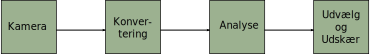
\includegraphics[scale=1]{images/pig-network}
	\caption{Procesnetværk til udskæring af svin på et slagteri.}
	\label{fig:pig-network}
\end{center}
\end{figure}



\subsubsection*{Implementering i Greenletsversionen}
Til at implementere eksemplet uden brug af af RTP-udvidelsen i \pycsp, kan vi oprette hvert svin som et objekt og tilknytte en deadline. Nu kan hver proces evaluere om svinet har overskredet sin deadline, i det tilfælde fjerne svinet, og stoppe den videre behandling. Det er ikke angivet hvordan hele processen startes, men vi antager der findes en form for detektor foran røngtenkameraet, der opfanger når et svin passere og som dermed  starter processen. 
Når detektoren starter hele processen, opretter den svineobjektet som den sender til Røngtenprocessen, samt sender en kopi direkte til udvælgelse og udskæringsprocessen. dermed ved processen at der ankommer et svin som den skal udskære, og hvis den inden deadline får en analyse af svinet, kan den træffe et begrundet valg om hvilken model der skal bruges,  men hvis ikke denne analyse findes, bruges blot standardmodellen. \CRef{fig:pig-network2} viser det endelige  netværk, hvor detektoren er introduceret, og som sender data til hhv. Røntgenprocessen og til Udvælgelse og udskæringsprocessen. 

\begin{figure}
 \begin{center}
  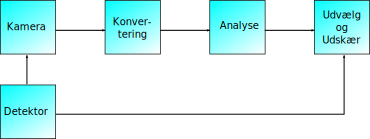
\includegraphics[scale=1]{images/pig-network2}
	\caption{Procesnetværk med detektor til initiering af hvert svin.}
	\label{fig:pig-network2}
\end{center}
\end{figure}

Et problem ved at implementere hele slagterieksemplet i \pycsp er  grænsefladen mellem verden hvor grisene kører på transportbåndet, og  greenletsversionen,  hvor  kun en proces kan være aktiv af gangen. Konvertering og analyse processen arbejder, mens  udskæringsprocessen venter på at svinene kommer inden for rækkevidde. Konvertering- og analysenprocessen  skal dog frivilligt afgive kontrollen, mens svinet er indenfor robottens rækkevidden og hvis de ikke gør, bliver svinet ikke udskåret. I stedet for at det samme system både skal foretage analysen som  styrer robotten, kan vi antage at processerne er mere autonome i deres opbygning. Dette giver at computeren der styrer robotten fungere uafhængigt af de computere der foretager konvertering og analysen. de to computere kan udveksle data igennem f.eks en database, harddisk eller anden delt datastruktur. Hvis analysen bliver færdig gemmes den, i den delte datastruktur, og robotten kan udnytte analysen, Hvis ikke den er klar bruges standard modellen.    



%\subsection{Eksempel 2 - Sensornetværk med høj/lav -prioritet}
%\inline{eks2: skal vise alternation, kan være en sensor som modtager måledata med lav prioritet og som skal sende måledata på opdordring med høj prioritet.}


\section{Design og implementering}
%\inline{Beskrivelse af design med udgangspunkt i eksemplet}
For at designe en implementering af simulering i diskret tid i \pycsp, skal vi foretage en række ændringer i forhold til den nuværende implementering. Specifikt skal vi ændre på planlægningen og eksekveringen af processer, hvortil vi har brug for at kunne repræsentere en diskret tidsmodel. Vi vil i dette afsnit gennemgå de relevante problemstillinger og løsningsmodeller samt give et overblik over, hvordan vi har valgt at implementere ændringerne rent praktisk i koden. 


\subsection{Kodestruktur}  
Efter i kapitel \ref{chap:csp} at have valgt at udvide \emph{greenlets}"-versionen, skal vi vælge hvordan vi ønsker at videreudvikle koden. Vi forventer at genbruge store dele af koden fra \emph{greenlets}"-versionen, og kun foretage udvidelser på enkelte afgrænsede områder. Desuden ønsker vi at isolere vores ændringer fra den originale \emph{greenlets}"-version. Med denne isolation forventer vi, at hvis/når der sker tilrettelser af \emph{greenlets}"-versionen af \pycsp, vil man ikke skulle foretage de samme tilrettelser i vores version. 
Isolationen mellem de to versioner skal opnås via nedarvning, således at det fra en brugers synsvinkel ser ud til, at vores version er fuldstændigt sepereret fra \emph{greenlets}"-versionen.

Hver af de tre versioner har sin egen mappe i \pycsp og i hver af disse findes en tilhørende \code{\_\_init\_\_.py} fil, der fungerer som et manifest for den givne version. Vi opretter vores egen version kaldet \emph{simulation} og opretter også en tilhørende mappe på samme niveau som de andre versioner og med sin egen manifestfil. Manifestfilen kan nu bruges til at udvælge de funktioner, der skal tages direkte fra \emph{greenlets}-versionen, og hvilke funktioner, der skal udvides og som derfor vil ligge i den nye mappe.

\begin{lstlisting}[float=hbtp,label=fig:init,caption=Uddrag af \code{\_\_init\_\_.py} for simulationsversionen.]
from guard import Timeout, Skip
from pycsp.greenlets.alternation import choice
from alternation import Alternation
from pycsp.greenlets.channel import ChannelPoisonException, ChannelRetireException
\end{lstlisting}

I \cref{fig:init} kan man se, at funktionerne \code{choice}, \code{ChannelPoisonException} og \code{ChannelRetireException} alle bliver hentet fra \emph{greenlets}"-versionen, mens funktionerne \code{Timeout, Skip} og \code{Alternation} bliver importeret fra samme mappe og derfor er modificerede versioner. For slutbrugeren  vil dette dog ikke være synligt, og han vil blot se \emph{simulation}"-versionen som en selvstændig version på lige fod med de andre tre versioner.

\subsection{\code{Scheduler}-klassen}
\label{sec:scheduler}
Med valget af \code{greenlets}"-versionen som grundversion, og med henblik på at hovedparten af vores ændringer vil være i \sched en, vil vi kort gennemgå dele af klassen \code{Scheduler}.

\begin{lstlisting}[firstnumber=132,stepnumber=5,numbers=left, float, label=fig:scheduling, caption=Uddrag af Scheduler.py i \emph{greenlets}versionen.]
    def getInstance(cls, *args, **kargs):
        '''Static method to have a reference to **THE UNIQUE** instance'''
        if cls.__instance is None:
            # (Some exception may be thrown...)
            # Initialize **the unique** instance
            cls.__instance = object.__new__(cls)

            # Initialize members for scheduler
            cls.__instance.new = []
            cls.__instance.next = []
            cls.__instance.current = None
            cls.__instance.greenlet = greenlet.getcurrent()

            # Timer specific  value = (activation time, process)
            # On update we do a sort based on the activation time
            cls.__instance.timers = []

            # Io specific
            cls.__instance.cond = threading.Condition()
            cls.__instance.blocking = 0
\end{lstlisting}

 I \cref{fig:scheduling} ses et uddrag af initialiseringskoden, der er interessant, fordi det er her alle de interne datastrukturer oprettes. Man kan her se de tre lister af processer, som \sched en har til rådighed til at varetage processkifte. 
 \begin{list}
 \tightlist 
 \item \code{new}: Initieres på linje 140 og består af processer, som lige er blevet planlagt for første gang. Nye processer kan ankomme til listen \code{new} via funktionerne \code{Parallel, Sequence} og \code{Spawn}.
 \item \code{next}: Initieres på linje 141 og indeholder de processer, der er klar til at blive kørt, og som har været kørt på et tidligere tidspunkt. Et eksempel kunne være en proces, der har stoppet sin kørsel for at vente på kommunikation. Processen vil blive placeret i denne liste, når kommunikationen er overstået. 
 \item \code{timers}: Initieres på linje 147 og indeholder de processer, der har tilknyttet en timeout. De skal først planlægges på et senere tidspunkt og venter dermed blot. Hvert element i listen består både af processen samt et tidsstempel for hvornår processen skal genaktiveres. 
 \item \code{blocking}: Initieres på linje 151 og er en variabel. Processer, der venter på IO-operationer, er ikke klar til at blive planlagt, men heller ikke afsluttet. \Sched en kan derfor ikke planlægge dem, men holder styr på antallet af ventende processer vha. denne variabel. Dette bruges bla. for at kunne afgøre om \sched en har planlagt alle processer.
\end{list}

Når \sched en er startet, gennemløber den alle tre lister gentagne gange, indtil de alle er tomme, og der ikke er nogle processer, der er blokeret. Dette betyder at der ikke længere kan komme nye processer til der ønsker at blive lagt på \sched en, og dermed kan den afslutte.

For at markere at vi ikke kun skal  planlægge rækkefølgen
af processerne, men også styre tiden, har vi lavet en
\code{Simulation}"-klasse, der arver fra \code{Scheduler}"-klassen. Alle ændringer
vi skal foretage for at kunne planlægge processer under hensyntagen til tid, vil således være indkapslet i denne klasse. 
Dette har yderligere den fordel, at man tydeligt kan se at alle klasserne i \code{simulation}-versionen arver en \sched~ fra \code{Simulation} og
ikke en \sched \xspace fra \code{greenlets}-versionen.

\subsection{Tid} \label{sec:tid}
For at kunne planlægge begivenheder i \des kræves det at alle processer og \sched en har en global forståelse af tid.  Det er derfor en af hjørnestenene i implementeringen af \des, hvordan tid introduceres til \pycsp.  
Begrebet tid er ikke en del af \csp, men er alligevel blevet introduceret i \pycsp, for  at  kunne tilknytte en timeout til en \code{alternation}. Vi ønsker
at videreudvikle denne struktur til at håndtere tid generelt for alle
processer, og til at fungere med vores tidsmodel, modsat den eksisterende
løsning, hvor \code{time}-modulet benyttes.
 
\CRef{Timeout} viser et eksempel på brugen af tid i det eksisterende \pycsp, hvor en \code{alternation} er villig
til at læse fra kanalenden \code{Cin} i 0,5 sekunder. Hvis ikke der
er modtaget en besked indenfor 0,5 sekunder, accepteres dens \code{timeout-guard},
og processen fortsætter sin kørsel uden at have læst fra kanalen.

\begin{lstlisting}[float=hbtp, 
label=Timeout,caption=Timeout i Alternation (fra dokumentationen til PyCSP)]
Alternation([{Timeout(seconds=0.5):None}, 
             {Cin:None}]).select()
\end{lstlisting}

Fra en brugers synsvinkel repræsenteres tiden internt i \pycsp som realtid, men dette er ikke korrekt. Helt generelt kan computere ikke håndtere kontinuerlige begreber, som realtid er, og \code{time}-modulet, der står for håndtering af tid i Python og dermed \pycsp, kan derfor ikke give brugeren mulighed for at benytte realtid. 

 I stedet tilbyder \code{time}-modulet det, vi vil kalde ``pseudo realtid'', der minder om realtid, men på en række områder afviger fra denne. Den største forskel mellem realtid og pseudo realtid er, at i computere kan tiden ikke være kontinuerlig, men må nødvendigvis være diskritiseret, og som oftest i et fast lille tidsskridt. Vi skal med vores diskrete tidsmodel derfor ikke foretage en konvertering fra kontinuerlig til diskret tid, men i stedet skal foretage en konvertering fra en diskret tidsmodel. hvor tiden stiger med et fast tidsskridt, til en diskret tidsmodel, hvor tiden stiger med variable tidsskridt. Vi skal desuden ændre fremskrivningen af tiden så den  drives af begivenheder og ikke af et eksternt modul, som i pseudo realtid. \fxnote{Kan vi ryste noget ud med hvorfor det er godt vi ikke skal gå fra kontinuerlig til diskret tid?}
 
 
\subsubsection{Sammenhæng mellem tidsintervaller i realtid og diskret tid}
Da man i \code{time}-modulet har et fast tidsskridt, og
realtiden også er inddelt i faste størrelser
som eks. sekunder, kan man med \code{time}-modulet måle tidsintervaller, der
korresponderer med realtiden. I \des findes der ikke en
sammenhæng til  realtiden, da tiden blot er et tal, der starter som 0, og stiger
i arbitrære tidskridt. Når tiden i \des på denne måde er afkoblet
en relation til realtid, giver det ikke mening at have elementer i simuleringen, der er afhængige af realtid. 
I \pycsp kan man planlægge en timeout til at ske om f.eks. 5 sekunder. I \des findes sekunder som
begreb ikke, men man  angiver i stedet, at når tiden er talt op med 5 tidsskridt, skal
begivenheden ske. Der findes dog ikke en total afkobling mellem tiden i \des og realtiden, for givet et konkret problem, der skal modelleres i \des, vil der altid være en sammenhæng mellem tiderne. Men da denne sammenhæng ikke er fast, skal den defineres eksplicit af brugeren, som f.eks at 5 sekunder i problemet defineres som en stigning i tiden med f.eks 5, 0,5 eller 0,05 i simuleringsmodellen.

Når tiden i \des er uafhængig af realtiden, er der ingen grund til at bruge en kompleks model af tiden, og vi har derfor valgt at repræsentere tiden som et positivt tal, der findes internt i \sched en. Dermed findes der kun en version af tiden, da  \sched en er en singelton. For processer, der ønsker at kende tiden, har vi
introduceret funktionen \code{Now}, der returnerer tiden fra \sched en, når funktionen kaldes. En fordel ved brugen af funktionen \code{Now} som en wrapperfunktion til at bede om tiden i forhold til den eksisterende kode, der direkte kalder \code{time}-modulet, er, at vi frigøres fra en konkret implementering af tid. For fremtiden er det kun funktionen \code{Now}, der skal omskrives, for at hele systemet bruger en anden implementering tid.

I den eksisterende kode har det ikke været tiltænkt, at man ønskede at udskifte implementeringen af tiden, vi skal derfor ændre de steder, hvor \code{time}"-modulet er refereret. Heldigvis bruges \code{time}-modulet kun ved udvælgelse af processer fra \code{timers}-listen (\cref{fig:green:timer}). 
\begin{figure}[hbtp]
\begin{minipage}[c]{\linewidth}
\begin{lstlisting}[firstnumber=204, label=fig:green:timer, caption=Udvælgelse af proces fra listen timers (fra scheduling.py)]
if self.timers and self.timers[0][0] < time.time():
  _,self.current = self.timers.pop(0)
  self.current.greenlet.switch()
\end{lstlisting}
\end{minipage}
\begin{minipage}[c]{\linewidth}
\begin{lstlisting}[firstnumber=124, label=fig:sim:timer, caption=Udvælgelse af proces fra listen timers (fra simulation.py)]
if self.timers and self.timers[0][0] <= Now():
  assert self.timers[0][0] == Now()
  _,self.current = heapq.heappop(self.timers)
  self.current.greenlet.switch()
\end{lstlisting}
\end{minipage}
\end{figure}
Her sammenlignes på linje 204 tidsværdi for den første proces i \code{timers} med det nuværende tidspunkt givet af \code{time}-modulet.
Hvis det nuværende tidspunkt er større end værdien i \code{timers}, udvælges denne proces til at køre næste gang og fjernes fra listen.
For at planlægge begivenheder præcist, skal processerne kunne eksekveres på et specifikt tidspunkt. Dermed har  \sched en i \code{simulations}-versionen behov for at kunne  styre aktiveringen af processerne på et finere niveau end, hvad der er muligt med \code{greenlets}"-versionen.  
I \code{simulation}"-versionen har vi fuld kontrol over tiden, da  den står stille, mens processerne eksekveres, hvorfor dette ikke er et problem.
Vi  tilføjer den begrænsning, at tiden skal være præcist det, der er angivet i \code{timers}, før processen skal aktiveres, og ikke kun større, som angivet i \code{greenlets}-versionen. \CRef{fig:sim:timer} viser udvælgelsen af en proces fra \code{timers} i \code{simulerings}-versionen ved brug af \code{Now}-funktionen, hvor tidspunktet skal være præcist det som processen har angivet.

\subsubsection{Fremskrivning af tid}
I pseudo realtid drives tiden frem af et eksternt modul for at efterligne realtid, der kontinuerligt stiger. I pseudo realtid fremskrives tiden derfor uafhængigt af processernes tilstand og derfor vil et program der med korte mellemrum beder om tiden, få et stigende tidspunkt. I \des  skal tiden i modsætning til realtid stå stille, når processerne er aktive, og kun i forbindelse med en planlagt begivenhed skal tiden drives frem til tidspunktet for denne begivenhed.

\fxnote*{skriv tegning}{Vi kan demonstrere, hvordan den kontinuerlige tid har indflydelse på  \pycsp med et eksempel}. Proces 1 har startet en ny tråd via \code{io-decoratoren} og er derfor blokeret. Proces 2 står i en \code{alternation} med en \code{timeout-guard}. Uafhængigt af den tid, det tager proces 1 at komme ud fra sit blokerede kald, skal proces 2 vide hvornår dens timeout er indtrådt. Dette er implementeret i \code{greenlets}-versionen i \cref{fig:blocking_sleep} på linjerne 242 til 251. Her startes en separat tråd, der vil signalere til \sched en, når tiden for næste begivenhed i \code{timers} listen indtræffer. \Sched en kan nu nøjes med at vente på et signal, som vil komme fra enten en blokeret proces eller den nyoprettede tråd.

Når tiden i \des ikke er drevet af en eksternt modul, er nødvendigheden af en ekstra tråd til  håndtering af tid irrelevant. Først når alle begivenheder til et tidsskridt er eksekveret, skal tiden i \des tælles op. Dette betyder i vores konkrete eksempel, at  så længe proces 1 er blokeret, står tiden stille, og  \sched en venter på dem. Vi kan ikke tælle tiden op, blot fordi nogle processer er blokeret af \code{io-decoratoren}, ligesom vi ikke kan tælle tiden op, så længe der er processer der er aktive. %blot mens nogle processer eksekvere en anden tilfældig funktion.

Først når alle processer venter i enten \code{timers} listen eller på kommunikation, kan der ikke ske flere begivenheder og tiden fremskrives. 
I dette tilfælde  kan \sched en finde tidspunktet for den begivenhed, der ligger tættest på det nuværende tidspunkt,  og springe frem til denne begivenhed. Dette er implementeret i \cref{fig:sim_sleep}.
\begin{figure}[hbtp]
\begin{minipage}[c]{\linewidth}
\begin{lstlisting}[firstnumber=239, label=fig:blocking_sleep, caption=Uddrag af \sched en i \code{Scheduler}]
self.cond.acquire()
if not (self.next or self.new):
    # Waiting on blocking processes or all processes have finished!
    if self.timers:
        # Set timer to lowest activation time
        seconds = self.timers[0][0] - time.time()
        if seconds > 0:
            t = threading.Timer(seconds, self.timer_notify)
            # We don't worry about cancelling, since it makes no 
            # difference if timer_notify is called one more time.
            t.start()
            # Now go to sleep
            self.cond.wait()
    elif self.blocking > 0:
        # Now go to sleep
        self.cond.wait()
    else:
        # Execution finished!
        self.cond.release()
        return
self.cond.release()
\end{lstlisting}
\end{minipage}
\begin{minipage}[c]{\linewidth}
\begin{lstlisting}[firstnumber=158, label=fig:sim_sleep, caption= Uddrag af \sched en i \code{Simulation}]
self.cond.acquire()
if not (self.next or self.new):
  # Waiting on blocking processes
  if self.blocking > 0:
    # Now go to sleep
    self.cond.wait()
  #If there exist only processes in timers we can increment
  elif  not (self.next or self.new or self.blocking): 
      if self.timers:
          # inc timer to lowest activation time
          self._t = self.timers[0][0]
      else:
          # Execution finished!
          self.cond.release()
          return
self.cond.release()  
\end{lstlisting}
\end{minipage}
\end{figure}


\subsubsection{Timeout} 
I \pycsp findes der, som nævnt i \autoref{chap:csp} en \code{alternation}, hvor brugeren har mulighed for at tilknytte to specielle guards. Den ene er en SKIP-guard, der giver mulighed for at kommunikere, hvis kanalen er klar, og ellers fortsætte uden at kommunikere. Den anden er timeout-guarden, der udvider SKIP-guarden, så man venter på kommunikation i en given periode, hvorefter man tager SKIP-guarden. 
Når \des indføres, ændres tiden, så timeout-guarden opererer på tidsskridt fremfor en tidsperiode. Vi går derved fra en situation hvor en timeout-guard f.eks. er villig til at vente i fem sekunder, til en situation hvor den er villig til at vente i 5 tidsskridt. Denne ændring virker umiddelbart simpel, men introducerer et problem i forhold til hvornår timeout-guarden vælges: En proces kan nu ønske at kommunikere i indeværende tidsskridt, men ikke i det efterfølgende. Vi kan dog ikke i tidsskridtet evaluere om kommunikation er muligt. Dette skyldes, at tiden står stille, mens processerne er aktive, så selvom kommunikation ikke er muligt på ét tidspunkt i tidsskridtet, så kan en efterfølgende begivenhed i samme tidsskridt muliggøre kommunikation.


En løsningsmodel på denne problemstilling kunne være at lade processer i timeout-guards vente helt frem til næste tidsskridt, og så her lade dem vælge SKIP-guarden. Dette efterfølgende tidsskridt kan enten være et ekstra skridt, vi introducerer specifikt for at håndtere disse timeout-guards, eller det kan være det næste tidsskridt, hvortil der er planlagt en begivenhed. 
Såfremt vi introducerer et kunstigt tidsskridt, skal dette specificeres i definitionen af timeout-guarden. Uanset hvor lille et tidsskridt vi specificerer, kan vi ikke garantere, at der ikke efterfølgende i samme tidsskridt vil blive planlagt en begivenhed, der skal indtræffe mellem indeværende tidsskridt og det kunstige tidsskridt, vi specificerede i timeout-guarden. Herved er der risiko for, at rækkefølgen af begivenheder, der skal udføres, bliver ændret, hvilket er uacceptabelt. 
Alternativt kan man vælge at lade tiden springe til den næste begivenhed, der er planlagt, og der som det første vælge SKIP-guarden. Her vil man ikke risikere at ændre på rækkefølgen, men derimod at springe for langt frem i tiden. Dette kan være et problem, hvis en proces, der tager en SKIP-guard, efterfølgende planlægger en begivenhed.
Begge muligheder har grundlæggende den svaghed, at oprindeligt ønskede man kun at kommunikere i det indeværende tidsskridt og ikke i hverken et vilkårligt lille tidsrum eller i et tilfældigt tidsrum frem til en efterfølgende begivenhed.

En sidste løsningsmodel er at vente til lige før, tiden tælles op, og der kalde de ventende processers SKIP-guards. 
For at kunne adskille hvilke processer, der har en begivenhed til et tidsskridt, og hvilke, der venter på kommunikation, kan vi \fxnote*{illustration}{benytte os af edge-triggering} til at dele hvert tidsskridt op i to grupper, henholdsvis wake-first og wake-last.
I wake-first-gruppen udføres de processer, der har tilknyttet en begivenhed til det givne tidsskridt, mens man i  wake-last-gruppen aktiverer SKIP-guarden for de processer, der venter på en timeout.

Edge-triggering er den bedste løsningsmodel af de beskrevne, da man her har mulighed for at udføre alle begivenheder, som måske resulterer i kommunikation, og først derefter aktivere SKIP-guards for de processer, der har en timeout til samme tidsskridt. Ulempen ved denne metode er at det kræver en mere kompleks implementering, da der nu findes to seperate måder at vente for hhv. begivenheder og timeouts.

\subsection{Funktionen \code{Wait}}\label{sec:Wait}
Vi har valgt at anskue planlægningen af en begivenhed til et bestemt tidspunkt, sådan at den proces der skal udføre begivenheden venter indtil tiden for begivnheden er nået, og først her begynde udførslen. Dette vil i praksis være det samme som en planlægning til tidspunktet men det letter implementeringen da vi ikke behøver nogen viden om specifikke begivenheder i vores \sched. 

\begin{lstlisting}[firstnumber=11 , stepnumber=2, numbers=left,float=hbtp, label=fig:simpy:yield, caption= Et yield i \simpy (taget fra Bank05.py i eksemplet fra \simpy)] 
def visit(self,timeInBank): 
  print now(), self.name," Here I am" 
  yield hold,self,timeInBank print now()
  self.name," I must leave" 
\end{lstlisting}
I programmeringssproget \simpy benytter man også denne metode med at lade en proces vente. Dette gøres ved at
foretage kaldet \code{yield}, som sørger for, at processen ikke
fortsætter, før et defineret tidsrum er gået. \CRef{fig:simpy:yield} viser, at en kunde er ankommet til banken, hvorefter kunden printer tiden, foretager et \code{yield}, printer tiden igen og afslutter.  Når processen har kaldt \code{yield}, er tiden steget med værdien af \code{timeInBank}. Grunden til at \simpy kan bruge \code{yield}, der er indbygget i Python og at dette kald afgiver kontrol over processen i et tidsrum, knytter sig til deres implementering af \simpy, hvor de bruger \code{corutine} som underliggende teknologi. Som standard kan  \code{corutine} afgive kontrollen med en proces via \code{yield}, og \simpy behøver derfor kun at sikre, at tiden er talt tilstrækkeligt op, før de returnerer til processen.

 Vi ønsker i \pycsp at have en lignende mulighed for at lade en proces vente. Med \code{greenlet}-modulet af brugertråde kan vi ikke bruge \code{yield}, da denne er specifik for \code{co-rutines}, men funktionaliteten er allerede delvist introduceret via \code{timeout} til \code{alternation} i \emph{greenlets}-versionen af \pycsp. Vi kan derfor bygge videre på denne funktionalitet med funktionen \code{Wait}, der fungerer som timeout, men som kan kaldes af processerne på et vilkårligt tidspunkt.

\begin{lstlisting}[firstnumber=20,float=hbtp, label=fig:wait, caption=Wait i \code{simulering}-versionen.] 
def Wait(seconds):
  Simulation().timer_wait(Simulation().current, seconds)
  t = Now()+seconds
  while Now()<t:
    p = Simulation().getNext() 
    p.greenlet.switch()
\end{lstlisting}

Funktionen \code{Wait} står for at kalde den interne funktion, der er lavet til timeouts, kaldet timer\_wait, hvorved processen lægges i \code{timers}-listen, og herefter sørge for først at returnere, når tiden er steget til det krævede. \code{Wait} er reelt det eneste værktøj, der skal til for at vente, og dermed planlægge begivenheder ud i fremtiden, og vi har på nuværenede tidspunkt en simpel \des, der kører i realtid. 

\subsection{Timers}  
I \pycsp bruges listen \code{timers} til at placere processer, der venter på en timeout i \code{alternation}. Dette er en niche feature ved \pycsp, som  sjældent bruges, og hvor der sjældent er samlet mange processer på en gang. 
I \cref{sec:Wait} beskriver vi hvordan processer, der ønsker at vente lægges på \code{timers}-listen, og i \cref{sec:tid} beskriver vi, hvordan \sched en kun tæller tiden op, når ingen processer kan foretage sig mere i et givent tidsskridt. Når tiden tælles op, vil  alle processer enten vente på kommunikation eller befinde sig i listen \code{timers}. De processer, der venter i en \code{alternation} og har tilknyttet en timeout, ligger begge steder. Gennemsnitslængden af listen vil derfor stige voldsomt og i vores version og dermed ændres kravene til hvilken  datastruktur der er bedst egnet. 
Med en kort, sjældent brugt liste vil omkostningerne til oprettelse og vedligeholdelse af en avanceret datastruktur være større end fordelene. Til vores skemaplanlægning  vil en min"-hob være det åbenlyse valg, da  man kan  indsætte elementer i konstant tid og fjerne det mindste element i $O(log\ n)$. Skemaplanlægning er specifikt nævnt i introduktionen til Pythons implementering\footnote{\url{http://docs.python.org/dev/3.0/library/heapq.html}} som eksempel på anvendelsesmulighederne for en hob. 

Da implementeringen af en hob allerede findes i Python i modulet \code{heapq}, som er effektivt implementeret i C, vælger vi at bruge denne. Den eneste handling,
der ikke er implementeret som standard, er fjernelsen af et arbitrært element fra hoben. Dette sker i den eksisterende løsning, når en proces
aktiverer et andet valg i \code{alternation} end timeout. I dette tilfælde skal
processen ikke vente på sin timeout, og derfor skal elementet fjernes fra \code{timers} listen. Her må man, som i
en normal liste, lave en lineær søgning i hoben og derefter genoprette
hob"-egenskaben i listen. Det vil dog ikke tage længere tid, da fjernelse af en timeout i \emph{greenlets}"-versionen på nuværende
tidspunkt bruger en lineær søgning, til at finde elementet der skal
fjernes, og genoprettelsen af hob"-egenskaben også kan gøres i lineær tid.

Det kræver ikke meget omskrivning for at konvertere en liste til en hob, hvilket ses ved at sammenligne \cref{fig:green:timer} linje 205 med \cref{fig:sim:timer} linje 126. 

\subsection{Annekteret kode fra \simpy.}
I vores implementering er der en del overlap med \simpy, da det har været en inspirationskilde til hvordan et simuleringssprog kan udvikles i Python. En del af arbejdet med \simpy har vi kunne bruge direkte i vore implementering efter devisen om ikke at genskrive eksisterende god kode. \simpy har en \code{Monitor}-klasse, der kan benyttes til dataindsamling, bearbejdning og visualisering. Denne klasse har vi i stor udstrækning genbrugt. Den fungerer ved at gemme en liste af tid/værdi par. Dermed kan man efter endt simulering, analysere  hvordan værdierne har ændret sig over tid. Klassen \code{Monitor} kan bruges direkte af brugere, hvor de selv  står for at at gemme værdier på passende tidspunkter igennem kørslen af programmet. Man ønsker tit at kende længden af en kø, der som oftest er implementeret via en liste. Vi har derfor lavet vores egen liste der kan indeholde en \code{Monitor}. Når længden af listen ændres, gemmes længden af listen i en montor til brug for senere analyse, uden brugeren selv skal stå det. Alternativt kan man lave en separat proces, hvis eneste formål er med en given frekvens at gemme listens længde. Fordelen ved denne løsning er at intervallet er jævnt fordelt, og man derfor lettere kan foretage tidsspecifik statistik.
 
\section{Evaluering}
  \inline{Evaluering af hvordan eksemplet løses efter den valgte 
  implementering benyttes. Inkluderer test+performance}
\subsection{Test af korrekthed}
  Vi har igennem designet og udviklingen af \code{simulerings}-versionen brugt en Test Driven Development (TDD). I TDD starter man med at skrive tests til en ny egenskab der skal udvikles. Designet er implementeret korrekt når testene kan gennemføres korrekt. Dette medfører at vi løbende i forbindelsen med udviklingen af \emph{simulerings}-versionen har skrevet tests. Desuden har vi integreret alle tests fra \emph{greenlets}-versionen ind i \emph{simulerings}-versionen, således at tests skrevet til \emph{greenlets}-versionen også tester vores version. Resultaterne af testene kan ses i tabel \fxerror{TODO! testene virker ikke:(}
  
\subsection{Eksempler}



\subsection{Effektivitet}  
\inline{skal vi overhoved evaluere performance?}
  


\section{Fremtidigt arbejde}
\section{Opsummering}

\chapter{Real-time planlægning}
Vi vil i dette kapitel beskrive Real-time planlægning (RTP), samt diskutere hvordan det kan implementeres i \pycsp. 

RTP er baseret på den kendsgerning at nogle begivenheder i programmer kan være vigtigere at få udført end andre indenfor en afgrænset tidsperiode. Dette kan f.eks. være interrupts, input- eller output enheder eller interne processer. Med RTP tilknytter man en deadline for hver begivenhed, som bruges til at planlægge rækkefølgen for afvikling af begivenhederne. Formålet er at optimere antallet af begivenheder der når at blive udført inden deres deadline er overskredet. Normalt anses alle begivenheder for at være lige vigtige, og de planlægges ud fra en optimal udnyttelse af processoren. Denne optimale processorudnyttelse kan man være nødt til at gå på kompromis med hvis man ønsker at bruge RTP og derved prioritere visse begivenheder højere end andre. Man kan forestille sig en situation hvor man ikke starter en begivenhed med lav prioritet selv om den er klar, hvis man ved at en begivenhed med høj prioritet er klar kort tid efter, og venter derfor på at den er klar og igangsætter begivenheden med høj prioritet med det samme. 
RTP benyttes meget i specialiserede indlejrede systemer til f.eks medicinsk udstyr, kontrol af luftrummet, på rumstationen ISS\cite{Audsley1990} og mange andre steder. Det er dog også anvendeligt i i mere gængse applikationer, typisk i forbindelse med en eller anden form for interaktion med den virkelige verden. 

I litteraturen omkring RTP bruges begreberne hard- og soft deadlines samt hard- og soft real-time systemer forskelligt, så vi vil i det følgende gennemgå hvordan vi definerer disse begreber. Vi har valgt at illustrere deadlines ved hjælp af time-value funktioner, hvor "værdien" indikerer det bidrag begivenheden bidrager med til systemets overordnede mål. 

\subsubsection{Kritisk deadline}
En kritisk deadline er en deadline som under alle omstændigheder skal overholdes for at opretholde systemets integritet. Såfremt en kritisk deadline overskrides vil der påføres skader på systemet som kan forårsage at systemets tilstand bliver udefineret. En kritisk deadline er illusteret i \cref{fig:hard-rtp}.

\begin{figure}
 \begin{center}
  \includegraphics[scale=0.75]{images/critical-deadline}
	\caption{Begivenhed med kritisk deadline.}
	\label{fig:hard-rtp}
\end{center}
\end{figure}


\subsubsection{Hard deadline}
Vi definerer en begivenhed til at have en hard deadline såfremt en færdiggørelse af begivenheden efter deadlinen ikke tilfører systemet nogen positiv værdi. Modsat en kritisk deadline kan en overskridelse af en hard deadline accepteres. I \cref{fig:hard-dl} vises en hard deadline for en begivenhed. 

\begin{figure}
 \begin{center}
  \includegraphics[scale=0.75]{images/hard-deadline}
	\caption{Begivenhed med hard deadline.}
	\label{fig:hard-dl}
\end{center}
\end{figure}
%Her tilføres der en positiv værdi til programmet hvis begivenheden afsluttes mellem dens starttidspunkt og dens deadline. Hvis begivenheden først er færdig efter deadline har den ingen værdi. En soft deadline (\cref{figure:soft-dl}) tilføjer den samme værdi som en hard deadline hvis begivenheden bliver færdig rettidigt. 

\subsubsection{Soft deadline}
Færdiggørelse af en begivenhed med en soft deadline til tiden tilføjer samme værdi til systemet som hvis den havde haft en hard deadline. Forskellen ligger i den tilførte værdi såfrem deadlinen overskrides. Hvor en hard deadline ikke tilføjer nogen værdi ved en overskridelse, vil en overskridelse af en soft deadline stadig tilføre en reduceret værdi ved færdiggørelse. Den tilførte værdi vil være omvendt proportional med længden af overskridelsen. \cref{figure:soft-dl} illustrerer en soft deadline. 

\begin{figure}
 \begin{center}
  
\includegraphics[scale=0.75]{images/soft-deadline}
	\caption{Begivenheden med soft deadline.}
	\label{figure:soft-dl}
\end{center}
\end{figure}


%Hvis deadlinen overskrides mindskes værdien den begivenhed tilføjer, omvendt propotionalt med overskridelsen. Ved en hard deadline er der ikke tilknyttet en egentligt %straf hvis en begivenhed ikke overholder sin deadline. Dette er derimod tilfældet i \cref{fig:hard-rtp}, der viser en begivenhed der tilføjer negativ værdi ved overtrædelse af en deadline. Hvis den tilknyttede straf for ikke at overholde en deadline er større end en hvad programmet maksimalt kan opnå ved at overholde alle deadlines kaldes det et ``hard real-time system''\cite{Laprie1989}.

\subsubsection{Hard real-time system}
Et hard real-time system er defineret ved et system der har begivenheder med hard deadlines, og kan garantere at disse ikke overskrides. Ydermere skal systemet være derterministisk, så denne garanti kan gives på forhånd. Det giver ikke mening at snakke om kritiske deadlines i hard realtime systemer da de kun adskiller sig fra hard deadlines med henblik på konsekvensen af en overskreden deadline, hvilket per definition ikke må ske i et hard real-time system.  

\subsubsection{Soft real-time system}
Et soft real-time system kan indeholde alle typer deadlines men opstiller ikke nogen garantier for at de overholdes. Det vil typisk bruge en algoritme til at op- og nedprioritere hvilke deadlines der skal overholdes såfremt alle deadlines ikke kan overholdes.\\
\\

Generelt vil der i et real-time system ikke være alle begivenheder der har den samme type af deadline. Nogle begivenheder har ingen deadline, nogle har en soft deadline, og få har en hard eller eventuelt en kritisk deadline. 
%For RTP skal kørslen planlægges så begivenhederne har den maksimale udnyttelse af tilgængelige ressourcer samtidigt med at så mange deadlines som muligt overholdes, hvor de vigtigte deadlines prioriteres højest. 

\section{Planlægning af begivenheder}
Planlægningen af hvilke begivenheder der skal køres hvornår, tager udgangspunkt i det overordnede formål med systemet. Generelt vil formålet være at minimere antallet af overskredne deadlines, men dette er sjældent det eneste kriterie der planlægges efter, ofte vil prioriteten for, og tiden det tager at udføre en begivenhed indgå i planlægningen. Eksempelvis vil man ofte prioritere at nå en kritisk deadline selv om det betyder at man overskrider to soft deadlines. 

%De fleste eksisterende real-time systemer arbejder på isolerede systemer, hvor planlæggeren har fuld kontrol over hele computeren. Derfor er hovedparten af forskningen indefor området gået til udarbejdelsen af specialiserede kerner og komplette operativsystemer\cite{damm1989real, jones1979staros, levi1989maruti,ramamritham14scheduling}. Vi ønsker i modsætning hertil ikke at udvikle en specialiseret kerne, men lade \sched en i \pycsp kunne planlægge processer efter bedste evne baseret på informationer den har om processerne.

For at foretage en planlægning af begivenheder der opfylder systemets formål bedst muligt, skal vi have så meget information om begivenheder som muligt - jo mere vi ved om dem jo bedre en planlægning kan der foretages. De relevante informationer i forhold til planlægningen er, hvornår en begivenhed forekommer, hvor lang tid den tager at udføre samt hvilken prioritet den har. 

Ud fra den tilgængelige viden kan der foretages en statisk eller dynamisk planlægning\cite{cheng1987scheduling}. Statisk RTP kræver at vi har alle de nævnte informationer om alle begivenheder. Herved kan vi på forhånd foretage en fuldstændig planlægning og allerede inden start have klarlagt om nogen deadlines vil blive overskredet. Såfremt vi ikke har alle informationer til rådighed, er vi nødsaget til at foretage en dynamisk planlægning. Dette vil ofte skyldes at vi enten ikke ved hvornår en begivenhed forekommer, eller at vi ikke har information om hvor lang tid der tager at udføre en begivenhed. I praksis vil det være svært at opstille eksakte værdier for hvor længe en begivenhed er om at blive udført og der benyttes derfor ofte estimater i stedet for. \fxnote{hvilken betydning har det at der benyttes estimater i stedet for eksakte værdier?}

%Overordnet kan begivenheder planlægges enten statisk eller dynamisk\cite{cheng1987scheduling}. I statisk RTP er alle begivenheder kendt på forhånd. Planlæggeren kan i dette tilfælde allerede inden start udregne om det er muligt at overholde alle deadlines. Alternativt planlægges begivenhederne dynamisk hvis der uregelmæssigt kan ankomme nye begivenheder der skal planlægges. 

%\fxnote{Motivationen her skal være at vi skal kende begivenheders frekvens og længde - skriv noget om det!}
%I realtidssystemer er næsten alle begivenheder cykliske, med enten en regelmæssig eller tilfældig frekvens. Begivenheder der forekommer med en regelmæssig frekevens kan være f.eks. være målinger der skal foretages med bestemte intervaller, hvor uregelmæssig frekvens ofte vil være tilfældet ved begivenheder der skal indtræffe som reaktion på udefrakommende input, f.eks. fejl eller alarmer. 

%\begin{shaded}
%Til planlægningen har planlæggeren behov for at vide hvor lang tid det vil tage at udføre en given begivenhed per periode, men da dette tal enten ikke er kendt eller fast for hver periode, bruges der ofte estimater. Dette medfører at en aperiodisk begivenhed kan ankomme på et vilkårligt tidspunkt og da planlæggeren kun har et estimat for tidsforbruget kan man  ikke tilknytte en ``hard deadline'' til aperiodiske begivenheder, da der altid findes en kæde af aperiodiske begivenheder der medfører en overskridelse af en deadline. 
%\end{shaded}

%\fxnote*{Dette skal måske flyttes eller omformuleres så vi ikke med det samme begrænses til dynamiske \sched}{I \pycsp kan der til alle tidspunkter tilføjes nye processer, og derfor vil vi kun beskæftige os med en dynamisk \sched. Desuden har man ikke med \pycsp fuld kontrol over hele operativsystemet. Mængden af processerkraft vi har til rådighed til kørsel af processerne vil derfor varriere uafhængigt af \pycsp, hvorfor vi heller ikke kan lave et pålidelig ``hard real-time system'', men fokusere på et ``soft real-time system''.}

\subsection{Metoder til skemaplanlægning}
Der findes adskillige metoder til at planlægge rækkefølgen af begivenheder. De adskiller sig fra hinanden med henblik på hvilke informationer der er til rådighed og hvad de optimerer efter. Vi har valgt at kigge på ``Rate monotonic algorithm''\cite{lehoczky1989rate,liu1973scheduling} og ``Earliest deadline first''\cite{liu1973scheduling} indenfor henholdsvis statisk og dynamisk skemaplanlægning.

Hvor processer isoleret set har behov for at udføre deres opgave inden deres deadline, har \sched en behov for kvantitativt at kunne organisere dem indbyrdes, således den til enhver tid kan vælge hvilken proces der skal udføres som den næste. Hovedformålet for en  \sched ~ er derfor at gå fra en række processer med tilknyttet deadline og eventuelt andre egenskaber til en prioriteret liste. \\
Der fokuseres i litteraturen på om en algoritme er stabil eller ej. Såfremt en algoritme er stabil vil man kunne definere en delmægnde af begivenheder, for hvilke man kan garanterer at de ikke overskrider deres deadline. 

\subsubsection{Rate monotonic algorithm (RM)}
RM er en statisk \sched, der fra start af udregner en prioriteret liste på baggrund af frekvensen af processens periode, dermed vil processer der oftet skal have udført deres periode en højere prioritet, end processer med lav frekvens. RM er todelt og i første del udføres før selve simuleringen udregnes  prioriteten for processerne, og udvælger hvilke processer der kan medtages i selve udførslen. Anden del står for udvælgelsen af processer  under simuleringen, og her vælges simpelt den proces med den højeste prioritet. 

Et problem for RM er at ved udvælgelsen af processer der kan medtages har man ikke en optimal udnyttelsen af processorkraft. \Citeauthor{lehoczky1989rate} er kommet frem til at ``worst-case'' er udnyttelsen i gennemsnit 88\\cite{lehoczky1989rate}. Et større problem i relation til implementering i \pycsp er dog at RM er dog at den er statisk. Til gengæld er algoritmen stabil ved en overskridelse af deadline for en proces. 

\subsubsection{Earliest deadline first (EDF)}
Som alternativ til den statiske \sched, hvor man ikke kan ændre prioriten af processen løbende gennem simuleringe, findes de dynamiske \sched er, hvor er EDF er et eksempel. Her evalueres prioriterne af processerne dynamisk igennem simuleringen og evaluere dermed løbende hvilke processer der skal udvælges. I EDF har den proces hvis deadline ligger tættest på højest prioritet og den hvis proces har længst til deadline den laveste prioritet. Aperiodiske processer kan i EDF indgå på lige fod med de periodiske da man til hvert processkift evaluere hvilken der har den nærmeste deadline, som både kan være en periodisk proces som en aperiodisk.

Udnyttelsen af processorkraft kan i EDF komme op på 100\, da alle processer bliver planlagt løbende i modsætning til RM der foretager et valg om en given proces kan planlægges.  Ulempen ved EDF er den ikke er stabil i det vi ikke har kontrol over hvilke processers deadline der bliver overskredet. Dette er specielt et problem hvis man har en en uhomogen samling processer hvor en mindre del er kritiske.

\subsubsection{Least Laxity(LL)}
LL er en modifikation af EDF. LL kigger på hvor lang tid en begivenhed tager at udføre sammenholdt med hvor lang tid der er til deadline for begivenheden. Laxity er defineret som deadline minus tiden det tager at udføre begivenheden. Laxity bliver altså et udtryk for hvor presserende det er at igangsætte en begivenhed for at den kan nå sin deadline. I LL bruges dette til at prioritere de begivenheder der har mindst laxity højest når begivenhederne planlægges. \\
\\
I systemer hvor begivenheder ikke er isolerede men kan have interne afhængigheder, kan der opstå det problem der hedder prioritetsinvertering\cite{sha1990priority}. Dette problem opstår hvis en begivenhed med høj prioritet er afhængig af en begivenhed med en lavere prioritet. Derved bliver begivenheden i praksis kørt med den lavere prioritet da den ikke er klar før begivenheden med lav prioritet er færdig. Problemstillingen kan vises klart med følgende eksempel. Forestil dig tre begivenheder ($B_0,B_1,B_2$)med prioriteterne $Pr_0>Pr_1>Pr_2$. Først udvælges $B_0$ da denne har højst prioritet, men stopper da den er afhængig af kommunikation fra $B_2$. Den næste begivenhed der udvælges vil være $B_1$, og dermed bliver $B_0$ unødigt forsinket mens $B_1$ kører.\\
En ofte benyttet metode til at undgå priotetsinvertering er priotetsnedarvning. Ved at benytte denne løsning vil en begivenhed med lav prioritet, som en begivenhed med høj prioritet er afhængig af, nedarve prioriteten fra den begivenhed der venter på den. Herved sikres det at begivenheder med høj prioritet ikke kommer til at vente unødigt på prioriteter med lav prioritet. \fxnote{flere løsninger på prioritetsinvertering bør nok nævnes.}

\section{Realtime planlægning i \pycsp}
Da vi ønsker at introducere RTP i \pycsp er der er række forhold som vi skal tage højde for. Vi vil i dette afsnit tage udgangspunkt i de ovenstående opstillede muligheder og sammenholde dem med \pycsp. 

begrænset forhåndsviden 
  dynamisk planlægning
  ingen viden om udførselstid - heller ikke estimater  

non-preemptive (snakkes der ikke om i foregående afsnit)

nedarvning 
  any->any kanaler kan potentielt give stor spredning af prioritet

\subsection{Priotetsnedarvning}
Skelne mellem read og write
måske skal en kanal arve prioritet?
hvornår skal prioriteten ændres? 

2 cases:
udvælgelse i alternation
propagering af prioritet

med nedarvning kan en proces uden deadline arve en høj prioritet uden at få sat en deadline. 

Skal processer der arver prioritet også arve deadline? Det skal de nok ikke, da de så kommer til at kaste exceptions selv på deadlines som brugeren ikke har sat. De skal nok kastes af den oprindelige proces med information om hvad den ventede på da den fejlede. 


\begin{shaded}
\subsection{Blokkerede processer}
I den teoretiske tilgang til RTP antages det ofte at processerne er periodiske, har en fast eksekverings tid per periode og er uafhængig af andre processer, og køres i et isoleret miljø. De forskellige tilgange til RTP fokuserer på hvordan man kan overvinde de enkelte antagelser ved isoleret og ophæve en af begrænsningerne. 


Dette er en højst idealiseret verden og i en introduktion af RTP i PyCSP vil processerne ikke overholde et eneste af disse antagelser. 
I \pycsp bruges rendezvous til at blokere kommunikerende processer.

Vi vil nu beskrive problemerne ved at processerne er afhængige af hinanden, og kan blokere hinanden, således at en proces med høj prioritet venter på processer med lavere prioritet. Forestil dig i \pycsp tre processer ($P_0,P_1,P_2$)med prioriteterne $Pr_0>Pr_1>Pr_2$. Først udvælges $P_0$ da denne har højst prioritet, men stopper da den skal kommunikere med $P_2$. Den næste proces der udvælges vil være $P_1$, og dermed bliver $P_0$ unødigt forsinket mens $P_1$ kører. Dette kaldes priority inversion\cite{sha1990priority}.

Der findes overordnet set to metoder til at løse problemet med priority inversion. Enten kan man ungå at blokerer processer, eller man kan benytte priority inherience\cite{sha1990priority}. Med \pycsp kan man ikke ungå at processer kommunikere, og dermed vil kunne blokere hvorfor priority inherience er den enste farbare vej hvis man skal sikre optimal planlægning.
\end{shaded}


  \section{Eksempel}
  \section{Design og implementation}
  \section{Evaluering}
  \section{Fremtidigt arbejde}
  \section{Opsummering}

\chapter{Interaktiv planlægning}
\label{chap:is}
\fxwarning{Mangler Evaluering}
\fxwarning{Mangler Opsummering}
Interaktiv planlægning (\is) er det sidste anvendelsesområde vi vil belyse med henblik på at indføre tid i \pycsp. Det har dog vist sig at emnet kun er sparsomt berørt i litteraturen, og der er ikke en klar definition på hvad det er og hvor det anvendes. 
%og at de få definitioner af \is vi har fundet, ikke er et selvstændigt anvendelsområde, men en definition af RTP med en hard deadline uden at være et kritisk system. \cite{?}. 
Vi forventede at dette anvendelsesområde var brugt i forbindelse med computerspil, men efter at have studeret litteraturen, og have rådført os med Lektor Kenny Erleben, der underviser på Det Danske Akademi for Digital Interaktiv Underholdning (DADIU), er vi kommet frem til der ikke findes en udbredt definition af \is. Han fortæller desuden at en af begrundelserne for at computerspilfirmaerne ikke er interesseret i at oplyse om deres metoder til at planlægge begivenheder i spil, er at det  betragtes som en  virksomhedshemmelighed. 

Vi vil derfor i stedet på baggrund af en række praktiske eksempler indkredse hvad vi forventer \is skal kunne bruges til, og på baggrund af eksemplerne se på muligheden for at implementere en model, så eksemplerne kan implementeres i \pycsp. Dette kapitel adskiller sig dermed væsentligt fra de foregående to kapitler, i og med tidsmodellen ikke baserer sig på en fast definition givet af litteraturen og vi ikke bygger på kendt viden.

\section{Eksempler}
Vi har valgt to scenarier som vi forventer med fordel kan benytte \is. Det første er en repræsentation af et ur, hvilket vi mener er det simpleste eksempel der kan gøre brug af \is. Det andet eksempel er en del af et computerspil, som er vores forventede primære anvendelsesområde for \is. 

\subsection{Et ur}
Det første eksempel på \is er en repræsentation af et digitalur. Uret består af fire cifre, og en gang i minuttet skal minuttallet tælles op. Det er et  krav at en opdatering af uret skal sætte uret til at vise det korrekte tidspunkt. Vi forestiller os at uret er en del af et større system hvor der er andre ressourcekrævende begivenheder der er vigtigere at få udført end opdateringen af uret. Opdatering af uret foregår ved at planlægge en begivenhed til hvert minut, der specificerer hvad uret skal vise. Da det har en lav prioritet, er der ikke er nogen garanti for at denne begivenhed indtræffer i det minut den er planlagt til. Derfor skal begivenheden  bortkastes såfremt den overskrider sin deadline. Deadlinen vil være det sidste sekund inden et nyt minut begynder, for at sikre den krævede korrekthed. 

Uret er repræsentativt for \is da der planlægges en række begivenheder der skal foregå i fremtiden, og hvor hver begivenhed også har tilknyttet en deadline.

\subsection{Computerspil}
Et andet eksempel vi mener repræsenterer  \is, er mere realistisk og bunder i vores oprindelige forventning om at \is  var defineret af computerspilindustrien, som en metode til at planlægge hvordan spil kan forløbe. Uden deres definition af \is vil vi i stedet opstille et hypotetisk eksempel. 

Vi forstiller os et computerspil, der er skrevet i \pycsp og hvor hvert element i spillet er en selvstændig proces. I dette computerspil skal der være en fugl, der jævnligt flyver på tværs af skærmen. Fuglen skal starte på et givet tidspunkt og med en fast hastighed bevæge sig over skærmen. Fuglens flugt over skærmen udregnes af to typer processer, baseret på en model der minder om videokomprimering. Den første procestype, er en højprioritets proces der står for udregne positionen af fuglen med  et fast interval. Den anden procestype kan bestå af mange lavprioritetsprocesser. Hver lavprioritetsproces står for en egenskab ved fuglen, som  f.eks. at justere fuglen i forhold til dens position, optimere animationen af fuglen, tilknytte fuglekvidren og andre ikke essentielle egenskaber. Den højtprioriterede proces udføres sjældent men er essentiel at få udført, mens lavprioritetsprocesserne blot skal udføres hvis der er mulighed for det og ellers skal droppes.

Uden tab af generelitet vil vi i dette eksempel begrænse os til at fokusere på en høj og en lavprioritets proces. Højprioritetsprocessen står for at beregne positionen mens lavprioritetsprocessen står for at flytte fuglen i forhold denne position.

\section{Beskrivelse}
Ud fra eksemplerne kan vi se på hvilke egenskaber de har, og hvilke krav de derved stiller for at kunne håndteres i et programmeringssprog. Først og fremmest ligger det inden for realtid ligesom RTP. Ligeledes skal der være mulighed for at tilknytte en deadline til en begivenhed. Dette vil i vores opstillede eksempler være hard deadlines, men vi kan ikke udelukke at der findes eksempler hvor andre typer deadlines vil være fordelagtige. Eksemplet med computerspillet viser at der er behov for at tilknytte en prioritet, der er uafhængig af deadline, til en begivenhed. Dette har vi diskuteret som en mulig udvidelse til RTP i \cref{sec:deadlineFuture}. Disse egenskaber minder alle om dem der er er givet for RTP. Ud over disse skal vi også kunne tilknytte et starttidspunkt til en begivenhed. Det lægger sig mere op af \des med det forbehold at vi i \is ikke garanterer at en begivenhed sker på et bestemt tidspunkt, men tidligst på det angivne tidspunkt.  

Vi kan dermed se \is som en blanding af RTP og \des, med tidsmodellen og deadlines fra RTP, og startidspunkter fra \des. 

%\is arbejder ligesom RTP i realtid. Desuden minder de også om hinanden da man i begge modeller arbejder med begivenheder, der har tilknyttet deadlines. For det tredje viser computerspilseksemplet at en udvikleren skal kunne tilknyttes prioriteter til begivenheder, der skal sættes uafhængigt af deres deadline i \is. Dette nævnte vi som en mulig udvidelse til RTP i \cref{sec:deadlineFuture}.

%\is og \des minder også om hinanden da man i begge modeller skal kunne planlægge en begivenhed til at foregå ud i fremtiden. Men hvor \des kan garantere at begivenheden sker på præcist det angivne tidspunkt kan vi i \is kun garantere at det sker efter et givent tidspunkt.

\section{Design og implementering} 
Vi argumenterer i kapitel \ref{chap:des} for at planlægning af begivenheder til et givet tidspunkt, kan tolkes som venten indtil tidspunktet. Vi kan derfor se \is som RTP med den yderligere mulighed at kunne vente. Som nævnt ovenfor vil det også være et krav at vi kan sætte en prioritet på en proces uafhængigt at processens deadline. 

Da kravene til \is rent teoretisk ligger meget tæt op ad de løsninger vi tidligere har beskrevet, vil vi også tage udgangspunkt i de allerede udviklede implementeringer. 

%I \des kom vi frem til at planlægningen af begivenheder ud i fremtiden også kan tolkes som en venten. Dermed kan man se på \is som en udvidelse til RTP, hvor man udover at have mulighed for at sætte en deadline skal have mulighed for at vente. For at kunne bruge RTP til \is vil det desuden være hensigtsmæssigt at  udvide RTP så det er muligt for udvikleren at tilknytte en prioritet til begivenheden.

\subsection{Funktionerne \code{Now} og \code{Wait}}
Som vi beskrev i \des introducerede vi de to globale funktioner \code{Now} og \code{Wait} der hhv. returnerer den aktuelle tid og lader en proces vente i et givent tidsrum. Vi har ændret den interne implementering af funktionerne, så de bruger realtid. Ved at genbruge de samme funktioner, sikres en ensartet implementering af tid på tværs af TimedPyCSP, og man kan i vores øjne med fordel tilføje dem til alle \pycsp versionerne, for på den måde at ensrette de forskellige implementeringer. Hvis \code{Now} og \code{Wait} blev inkluderet i \code{greenlets}-versionen kunne de fjernes helt i \is, da de to baserer sig på den samme tidsmodel.

For at benytte realtid i forhold til diskret tid bruger vi pythons \code{time} modul. Genimplementering består derfor kun i at ændre funktionen \code{Now} til at bede \code{time}-modulet om tiden i stedet for \sched en.

\subsection{Udvikler"-prioriteter}
I computerspilseksemplet, har processerne forskellige prioritet dikteret af udvikleren. Denne prioritet er ikke det samme som den prioritet der allerede findes i RTP, da denne  er beregnet af \sched en. For at adskille dem vil vi kalde prioriteterne der er angivet af udvikleren for udvikler-prioritet. Vi skal udvide RTP således at det kan håndtere processer, der både kan have deadlines og udvikler"-prioriteter tilknyttet. Dette har vi allerede beskæftiget os med i \cref{sec:deadlineFuture}, som en fremtidsmulighed, og passer derfor godt sammen med RTP.

Først skal det fastlægges i hvilket interval udvikler-prioriteter kan antage. Vi ønsker ikke at begrænse udvikleren ved at have for få prioriteter, men omvendt reduceres \sched ens  mulighed for at udvælge processer hvis hver proces har sin egen unikke prioritet. Hvis en udvikler kan vælge mellem et stort antal prioriteter risikere man også at introducere en prioritetsskrue. Dette sker hvis en udvikler flere gange undervejs i udviklingen af et program øger den maksimale prioritet, da han mener sin nuværende proces er den vigtigste uden at gennemtænke det i relation til alle andre processer. Dermed risikere man at udvande prioriteten de allerede udviklede processer.  Der skal derfor være en maksimal prioritet, og intervallet man kan angive prioriteter i, må ikke være så stort at processerne for unikke prioriteter.

Præcis  hvor stort intervallet skal være for udvikler"-prioriteter, kræver dog en bredere analyse af flere projekter, og vi vil derfor begrænse os til at lave et foreløbigt interval på ti, man senere nemt vil kunne ændre baseret på en bedre analyse.


I \code{RTP}-versionen er \sched en en EDF algoritme, som kun planlægger processerne på basis af deres deadline. Vi kan derfor ikke bruge den samme skemaplanlægningsalgoritme, men skal udvide \sched en. For at udvide \sched en skal vi definere den indbyrdes relation mellem deadlines og udvikler"-prioriteter. Baseret på eksemplet kan vi se at de processer der har  tilknyttet en udvikler"-prioritet skal gå forud for både de processer der har tilknyttet en deadlines og dem uden noget. 

I RTP  indeholder \sched en alle processer med en prioritet i en enkelt hob kaldet \code{has\_priority}. Vi kan enten udvide denne hob til en liste af hobe, en for hver prioritet. Med en liste af hobe vil hver hob være mindre og dermed vil de enkelte operationer på hoben være hurtigere. \Sched en kan desuden bruge EDF på hver hob da alle processerne i hver hob har samme prioritet. Til at udvælge hvilken hob der skal udvælges en proces fra løbes listen igennem efter den hob med de højst prioriterede processer, der har elementer. 

Alternativt kan vi udvide den ene hob, der allerede findes så alle processer, både med og uden udvikler"-prioritet befinder sig i den samme hob. Med denne metode kan man ikke bruge EDF, men der skal udvikles en  funktion der kombinere  udvikler"-prioriteten og deadlinen, til en endelig prioritet. Man vil så kunne bruge en Least Priority First (LPF) algoritme, der fuldstændigt svare til EDF, men bruger prioritet til at basere udvælgelsen. I sagens natur vil denne hob  være større end hvis man brugte en liste af hobe. Dette er dog ikke et stort problem, da hoben gemme data i en træstruktur og  søgetiden vokser derfor logaritmisk til antallet af elementer. Vi antager derfor at forskellen mellem de to fremgangsmåder ikke vil være nævneværdig, og under alle omstændigheder, vil den ikke være anderledes end i \code{RTP}-versionen, hvor der også kun findes en hob. Fordelen ved kun at bruge en hob er at vi kan genbruge \code{has\_priority} hoben, og  ikke skal lave en større omskrivning af \code{RTP}-versionen. Desuden skal vi ikke lineært gennemløbe en liste af hobe for at finde den først hob med elementer, men kan med det samme starte i den korrekte hob. Endnu en fordel ved denne metode er at vi nemt kan  ændre vores oprindelige antagelse om at prioritet skal gå forud for deadlines, blot ved at ændre på den eksterne funktion der kombinere de to parametre.

Vi mener at fordelene ved kun at have en hob, og muligheden for at kunne ændre på vægtningen af forholdet mellem udvikler-prioritet er større end besparelsen i tid ved at have flere hobe der skal vedligeholdes. Derfor vælger vi  at genbruge bruge \code{has\_priority}, som den eneste hob til  processer der har deadlines og udvikler"-prioritet. Med kun en hob skal vi derfor udvikle en ekstern funktion der kombinerer to tal til en endelig prioritet. Det kombinerede tal skal have den egenskab altid at udvikler"-prioriteten har forrang. Hver at bemærke er at des højere udvikler-prioriteten er des vigtigere er processen. I implementeringen af \code{has\_priority} bruges der en min-hob, hvorfor vi internt invertere udvikler"-prioriteten, så 0 er den højeste prioritet, og processer, hvor udvikleren ikke har angivet en prioritet, sættes til 10.

Vi valgt at implementere en simpelt løsning, hvor  de to tal lægges efter hinanden. Hvis man eksempelvis har en udvikler"-prioritet på 2 og en deadline på 20, sættes de efter hinanden så den endelige prioritet bliver 220. Dette kan vi gøre da antallet af cifre i hhv. deadlines og udvikler-prioritet ligger fast, så vi ikke risikere en forskydning, når de ligges efter hinanden. For at sikre at processer der har en udvikler"-prioritet, men ingen deadline også kan planlægges, bruges der en kunstig høj deadline. Man vil i vores løsning nemt kunne ændre på måden hvordan de to tal kombineres, blot ved at ændre i en funktion. 


% dikterede valget af \sched at priorite


    
\section{Evaluering}
\section{Fremtidigt arbejde}
Noget om mulighederne for at lave det i proces-versionen af \pycsp.
\section{Konklusion}

%\begingroup
%\setsecnumdepth{part} 
\chapter{Konklusion} 
\label{chap:konklusion}

Vores mål med dette speciale var, at undersøge muligheden for, at lave en udvidelse af \pycsp, der muliggør brugen af tid direkte i sproget. Der findes allerede et massivt teoretisk arbejde indenfor området, men ingen praktisk anvendelige implementeringer, så vores fokus har været på, at det skulle være praktisk anvendeligt. Dette afspejles ved, at vi har valgt at benytte eksempler som omdrejningspunkt for vores analyser af de tre anvendelsesområder. 

De tre anvendelsesområder vi identificerede i introduktionen var diskret simulering, realtids-planlægning og interaktiv tid. Vi har gennem vores analyse kommet frem til at det er mere hensigtsmæssigt at anskue anvendelsesområderne ud fra hvilken tidsmodel de bygger på. \CRef{fig:timemodel} viser således opdelingen af anvendelsesområderne i henholdsvis diskret og realtid.

\begin{figure}[htp]
 \begin{center}
  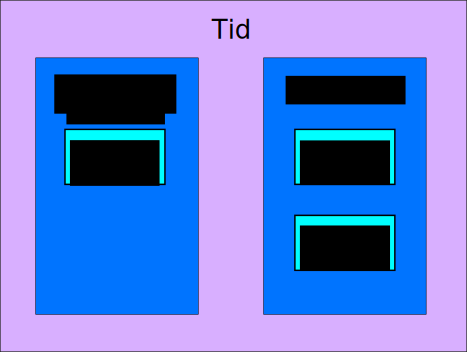
\includegraphics[scale=0.6]{images/timemodel}
	\caption{Forholdet mellem de tre anvendelsesområder af tid vi opstillede i introduktionen.}
	\label{fig:timemodel}
\end{center}
\end{figure}

Indenfor diskret simulering har vi udviklet en løsning, der er let at anvende, og som eliminerer kravet om en delt datastruktur for at administrere tid i \pycsp. Yderligere kræver løsningen væsentligt mindre kode til at administrere tiden, end en tilsvarende løsning lavet i ren \pycsp. 
Sammenligner vi vores løsning med \simpy, der er et framework til simuleringer, skrevet i Python, mener vi at vores løsning er mere intuitiv og fleksibel at benytte, til at modellere et givet problem. Dette tillægges i høj grad at vi direkte kan benytte \pycsp's processer og kanaler. Et eksempel på hvordan diskret simulering i \pycsp giver udvikleren større frihed til sin modellering finder vi i en kommende udvidelser til \simpy. De arbejder  på at udvide deres framework til at kunne håndtere reservation af flere begrænsede ressourser som skal benyttes samtidigt. Dette er allerede muligt i vores løsning, uden det har været vores fokus, da ressourcer blot modelleres som processer i \pycsp. Ønsker man at reservere flere ressourcer, kommunikerer man blot med flere processer, og når alle processerne har svaret, holder man alle de begrænsede resourcer. Arbejdet kan nu udføres, og ressourcerne frigives igen. 

I vores løsning til realtidsplanlægning har vi implementeret EDF, som den grundlæggende algoritme til at bestemme rækkefølgen, for udførsel af processer. Vi har implementeret prioritetsnedarvning for at imødekomme problemer med prioritetsinvertering, samt indført en prioriteret udvælgelse i \code{alternations} og når der kommunikeres over kanaler. Vores eksempel viser tydeligt at vores RTP-løsning kan gøre en forskel, såfremt der i programmet, kan foretages en differentiering i prioriteten af de processer der skal afvikles. 

Vi er kommet frem til at interaktiv planlægning ikke kan anses som et selvstændigt anvendelsesområde, men nærmere som en gren af realtidsplanlægning. De benytte begge realtid som tidsmodel, og har deadlines og prioriteter. Interaktiv planlægning har yderligere tilføjet et starttidspunkt, men det ændrer ikke fundamentalt på modellen. 

Vores løsninger er brugbare i den nuværende form, men der kan foretages en række udvidelser der vil gøre dem endnu mere anvendelige. 
Indenfor \des synes vi det kunne være spændende at udvide løsningen til at kunne foretage en dynamisk evaluering af køer, for derved at give ekstra fleksibilitet i de udviklede simuleringer. I RTP har vi lavet en basisimplementation der benytter EDF. Det kunne være interessant at kigge på mulighederne for at bedømme en proces' udførselstid, eller lade udvikleren angive dette. Det vil åbne op for brug af andre algoritmer end EDF, hvorved der åbnes op for brug af adskillige andre algoritmer til skemaplanlægningen og udvider anvendelsesområdet.  

%lettere at modellere processer
%Simpy kan ikke reservere begrænsede ressourcer

%Sammenligning med Simpy her 

%Tidsmodeller/anvendelsesområder

%Praktisk anvendelig implementering

%nuværende tilstand for anvendelsesområderne

%\endgroup 

 
%%%%%%%%%%%%%%%%%%%%%%%%%%%%%%%%%%%%%%%%%%%%%%%%%%%%%%%%%%%%%%%%%%%%%


\SingleSpacing
\fxerror{Check at sidetallet på litteraturlisten passer}
\printbibliography
\newpage
%\backmatter
\appendix

\pagenumbering{Roman}
\restorepagenumber
\chapter{Testresultater}


\section{Testresultater for \des}
\label{app:des-test}
\begin{longtable}{lr}
   	\toprule
    \mc{Test} & \mc{Resultat} \\
    \midrule
    \endfirsthead 
    \toprule
    \mc{Test} & \mc{Resultat} \\
    \midrule
    \endhead % slut efterfølgende headere
    \bottomrule
    \multicolumn{2}{r}{\textit{fortsættes}}
    \endfoot % slut footer
    \bottomrule
    \endlastfoot % slut sidste footer
    Doctest: simulation.Simulation & ok\\
    Doctest: simulation.io & ok\\
    Doctest: guard.testsuite & ok\\
    Doctest: alternation.Alternation & ok\\
    Doctest: alternation.testsuite & ok\\
    Doctest: channel.Channel & ok\\
    Doctest: channel.testsuite & ok\\
    Doctest: process.Parallel & ok\\
    Doctest: process.Spawn & ok\\
    Doctest: process.test\_suite & ok\\
    test\_alternation (test\_simulation.SimulationTestCase) & ok\\
    test\_buffer (test\_simulation.SimulationTestCase) & ok\\
    test\_buffered\_channels (test\_simulation.SimulationTestCase) & ok\\
    test\_decompose (test\_simulation.SimulationTestCase) & ok\\
    test\_io (test\_simulation.SimulationTestCase) & ok\\
    test\_timers1 (test\_simulation.SimulationTestCase) & ok\\
    test\_timers2 (test\_simulation.SimulationTestCase) & ok\\
    test\_timers3 (test\_simulation.SimulationTestCase) & ok\\
    test\_timers\_time\_in\_past (test\_simulation.SimulationTestCase) & ok\\
    test\_wait (test\_io.TestCase) & ok\\
\end{longtable}


\newpage
\section{Testresultater for RTP}
\label{app:rtp-test}
\fxnote{RS: ret stavefejl og sørg for at de to tabeller er formatteret ens}
\begin{longtable}{lr}
   	\toprule
    \mc{Test} & \mc{Resultat} \\
    \midrule
    \endfirsthead 
    \toprule
    \mc{Test} & \mc{Resultat} \\
    \midrule
    \endhead % slut efterfølgende headere
    \bottomrule
    \multicolumn{2}{r}{\textit{fortsættes}}
    \endfoot % slut footer
    \bottomrule
    \endlastfoot % slut sidste footer
test\_Alternation  & ok\\
test\_AlternationChoiseReader  & ok \\
test\_AlternationChoiseWriter  & ok \\
test\_AlternationExecuteReadDeadline  & ok\\
test\_AlternationExecuteSkipDeadline  & ok\\
test\_AlternationExecuteTimeoutDeadline  & ok \\
test\_AlternationExecuteWriteDeadline  & ok \\
test\_Alternationchoise1Deadline  & ok \\
test\_Alternationchoise2Deadline  & ok \\
test\_ChoisemultipleReader  & ok \\
test\_ChoisemultipleReader2  & ok \\
test\_ChoisemultipleWriter  & ok\\
test\_PoisonAndDeadline1  & ok\\
test\_PoisonAndDeadline2  & ok\\
test\_Reader\_Inheritance  & ok\\
test\_RetireAndDeadline  & ok\\
test\_Writer\_Inheritance  & ok\\
test\_channelpriority\_from\_low\_deadline  & ok\\
test\_channelpriority\_from\_low\_deadline2  & ok\\
test\_channelpriority\_from\_no\_deadline  & ok\\
test\_channelpriority\_from\_no\_deadline2  & ok\\
test\_readDeadline  &ok\\
test\_writeDeadline  & ok\\
test\_xreset\_inheritance  & ok\\
test\_xreset\_inheritance\_from\_two\_step  & FAIL\\
\end{longtable}


\fxwarning{inkluder kodeeksempler som best practice}


\chapter{Eksempler}
\section{Best practice for \des}
\lstinputlisting[label=code_wator, caption=WaTor i \code{simulerings}-versionen]{../projects/wator/wator-des.py}
\lstinputlisting[label=code_wator, caption=Simpelt bankeksempel i \code{simulerings}-versionen]{../projects/bank/src/bank03.py}
\lstinputlisting[label=code_wator, caption=Avanceret bankeksempel i \code{simulerings}-versionen]{../projects/bank/src/bank04.py}

\section{Best practice for RTP}  
\lstinputlisting[label=code_wator, caption=Slagterieksemplet \code{RTP}-versionen]{../projects/porks-rtp/porks-rtp.py}
\section{Best practice for IP}  
\lstinputlisting[label=code_wator, caption=Ureksemplet \code{RTP}-versionen]{../projects/watch-ip/watch.py}


\end{document}
